\chapter{Methodology}
\label{ch:method}

%───────────────────────────────────────────────────────────────────────────────
\section{System overview}
\label{sec:overview}

The system provides safe bimanual teleoperation of a PAL TRIAGo (two 7-degree-of-freedom (DOF) arms, a 7-DOF sensorised head, mobile base) through a Haption Desktop 6D Compact haptic interface (6~DOF), with shared-autonomy intent prediction, reference-level blending, and haptic guidance.
The architecture is factored into four decoupled real-time loops (Fig.~\ref{fig:arch}):
\begin{enumerate}[nosep]
\item a \textbf{quadratic program (QP)-based safety controller} running at control rate $f_{\text{ctrl}}$ (Appendix~\ref{app:config}), enforcing collision and joint-limit invariants on both arms simultaneously;
\item a \textbf{shared-autonomy inference layer} maintaining a discounted belief score over a discrete goal set, computing per-goal optimal policies, and arbitrating authority between the operator and the autonomy through the \emph{reference-level blending} channel~\cite{dragan2013policy,javdani2018hindsight,losey2018review};
\item a \textbf{haptic force-feedback layer} rendering the inferred intent as guidance forces on the operator's device through the \emph{haptic guidance} channel;
\item a \textbf{head perception layer} that both (a)~servoes the camera to keep the operator's active hand framed during teleoperation, and (b)~autonomously builds a camera-derived model of the tabletop scene that can replace the static world model as the source of the safety controller's collision barriers.
\end{enumerate}
Assistance reaches the operator through these two orthogonal channels --- reference-level blending and haptic guidance --- which are additive rather than alternative, so both can be active at once, and which, crossed with the two teleoperation control modes, form the $2\times3$ condition matrix. No loop shares a decision variable with another, so each loop's guarantees are self-contained. The operator-side half --- the device interface, the two teleoperation control modes, and the per-mode assistance strategies --- is developed later in this chapter; its cross-condition fairness properties are treated as a design feature in their own right and are evaluated in the user study.

\begin{figure}[t]
\centering
\resizebox{\linewidth}{!}{%
\begin{tikzpicture}[
  font=\footnotesize,
  >=Latex,
  blk/.style={draw=black, line width=0.5pt, rounded corners=2pt, align=center,
              fill=white, inner sep=2pt, minimum height=8mm, minimum width=#1},
  blk/.default=20mm,
  hum/.style={draw=black, line width=0.5pt, ellipse, align=center, fill=white, inner sep=2pt},
  core/.style={->, draw=black, line width=0.5pt},
  optB/.style={->, draw=orange!85!black, densely dashed, line width=0.7pt},
  optF/.style={->, draw=orange!85!black, densely dotted, line width=0.8pt},
  selArr/.style={->, draw=black!60, densely dashed, line width=0.5pt},
  lab/.style={fill=white, inner sep=1pt},
  tagl/.style={font=\footnotesize\bfseries, orange!85!black},
  grp/.style={line width=0.7pt, rounded corners=4pt, inner sep=3.4mm},
  gtitle/.style={font=\footnotesize\itshape, anchor=south},
]

% ---------------- operator side ----------------
\node[hum, minimum width=18mm, minimum height=8mm] (operator) at (0.6,15.0) {Operator};
\node (device) at (0.6,12.2) {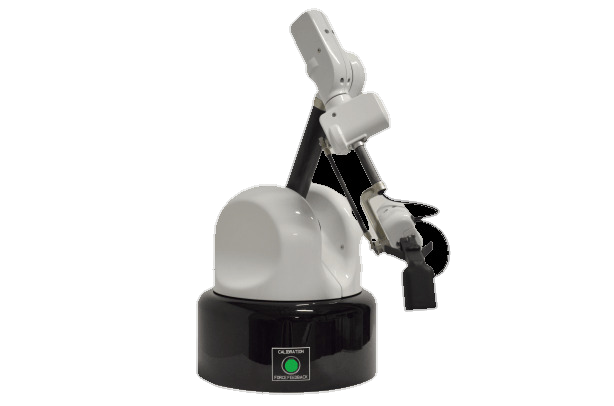
\includegraphics[width=22mm]{desktop-6D-compact-force-feedback-device-white.png}};
\node[lab, below=0mm of device] {Haptic device};
\draw[core] (0.95,14.6) -- node[right, lab]{$p_h, R_h$} (0.95,13.25);
\draw[core] (0.25,13.25) -- node[left, lab]{$w_h$} (0.25,14.6);

\node[blk=23mm] (fr)  at (4.4,13.3) {Force\\rendering};
\node[blk=23mm] (map) at (4.4,11.5) {Teleoperation\\mapping};
\begin{pgfonlayer}{background}
\node[grp, fit=(map)(fr), fill=black!3, draw=black!45] (tgrp) {};
\end{pgfonlayer}
\node[gtitle, black!60] at (tgrp.north) {Teleoperation};
\draw[core] (1.75,11.5) -- node[above, lab, align=center]{$p_h, R_h$\\$v_h,\omega_h$} (map.west);
\draw[core] (fr.west) -- node[above, lab]{$w_h$} (1.75,13.3);

% ---------------- shared autonomy ----------------
\node[blk] (intent) at (8.5,13.3) {Intent\\estimation};
\node[blk] (pol)    at (11.8,13.3) {Goal\\policies};
\node[blk] (arb)    at (10.15,11.5) {Arbitration};
\begin{pgfonlayer}{background}
\node[grp, fit=(intent)(pol)(arb), fill=orange!7, draw=orange!55!black] (sagrp) {};
\end{pgfonlayer}
\node[gtitle, orange!55!black] at (sagrp.north) {Shared autonomy};

\draw[core] (pol.west) -- node[above, lab]{$\pi_k^{\text{user}}$} (intent.east);
\draw[core] (map.east) -- node[below, lab, pos=0.3]{$v_{\text{user}}$} (arb.west);
\draw[core] (7.95,11.5) -- (7.95,12.9);
\draw[optB] (9.0,12.9) -- node[left, lab, pos=0.4]{$b_k$} (9.65,11.9);
\draw[optB] (11.3,12.9) -- node[right, lab, pos=0.4]{$\pi_k$} (10.65,11.9);
\node[tagl] at (10.15,12.65) {B};
\draw[optF] (intent.west) -- node[above, lab]{$b_k,\pi_k^{\text{user}}$} node[below=1pt, tagl]{F} (fr.east);

% ---------------- safety controller ----------------
\node[blk] (gov)   at (14.6,9.0) {Reference\\limiter};
\node[blk] (qp)    at (14.6,7.3) {\mbox{CLF--CBF QP}};
\node[blk] (col)   at (14.6,5.6) {Collision\\manager};
\node[blk] (sched) at (11.0,9.0) {Slack\\schedule};
\begin{pgfonlayer}{background}
\node[grp, fit=(gov)(qp)(col)(sched), fill=blue!6, draw=blue!45!black] (sfgrp) {};
\end{pgfonlayer}
\node[gtitle, blue!45!black] at (sfgrp.north) {Safety controller};

\draw[core] (arb.east) -- node[above, lab, pos=0.5]{$x_{\text{ref}}, \dot{x}_{\text{ref}}$} (14.6,11.5) -- (gov.north);
\draw[core] (gov) -- node[right, lab]{$x_g, v_g$} (qp);
\draw[core] (col) -- node[left, lab]{$J_{\text{soft}}, h_{\text{soft}}, d_{\text{safe}}$} (qp);
\draw[core] ($(qp.west)+(0,0.2)$) coordinate (qlam) -- node[above, lab, pos=0.4]{$\lambda_{\text{cbf}}, \lambda_{\text{jl}}$} (qlam -| {$(sched.south)+(-0.4,0)$}) -- ($(sched.south)+(-0.4,0)$);
\draw[core] ($(sched.south east)+(-0.2,0)$) -- node[above right, lab, inner sep=0.5pt, pos=0.55]{$w_{\delta}$} ($(qp.north west)+(0.3,0)$);

% ---------------- robot ----------------
\node (robot) at (5.2,6.9) {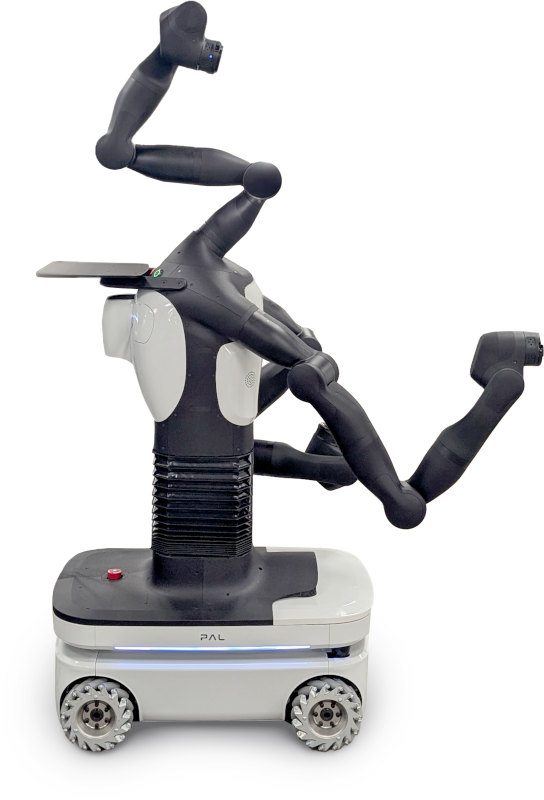
\includegraphics[width=20mm]{triago.png}};
\node[lab, left=0mm of robot] {TRIAGo};
\draw[core] ($(qp.west)+(0,-0.2)$) coordinate (qdot) -- node[below, lab, pos=0.9]{$\qdot^{\star}$} (qdot -| 6.2,0);
\draw[core] (col.west -| 6.2,0) -- node[below, lab, pos=0.25]{$q,\ \qdot^{\text{meas}}$} (col.west);

% ---------------- perception and world ----------------
\node[blk] (head)  at (5.2,2.6) {Head\\perception};
\node[blk] (perc)  at (9.0,2.6) {Perceived\\world};
\node[blk] (decl)  at (12.6,2.6) {Declared\\world};
\begin{pgfonlayer}{background}
\node[grp, fit=(head)(perc)(decl), fill=black!4, draw=black!45] (pwgrp) {};
\end{pgfonlayer}
\node[gtitle, black!60, anchor=north] at (pwgrp.south) {Perception and world};
\draw[core] (robot.south) -- node[right, lab]{RGB-D image} (head.north);
\draw[core] (head.east) -- node[above, lab]{$\hat{\mathcal{O}}$} (perc.west);
\coordinate (wsel) at (10.8,3.9);
\draw[selArr] (perc.north) |- (wsel);
\draw[selArr] (decl.north) |- (wsel);
\fill[black!60] (wsel) circle (0.6mm);
\draw[core] (wsel) -- (10.8,4.5) -- (18.1,4.5) -- node[right, lab, pos=0.5]{$\mathcal{G}$} (18.1,14.4) -- (11.8,14.4) -- (pol.north);
\draw[core] (14.6,4.5) -- node[right, lab]{$\mathcal{O}$} (col.south);
\draw[core] (col.east) -- (16.4,5.6) -- node[right, lab, pos=0.5]{$J_{\text{safe}}, b_{\text{safe}}$} (16.4,13.3) -- (pol.east);

\end{tikzpicture}}
\caption{System architecture. Ellipses and pictures are the human and physical endpoints, rounded rectangles are software nodes, grouped by layer. The operator sets the pose $(p_h, R_h)$ of the haptic device's handle, whose pose and twist $(v_h, \omega_h)$ the teleoperation mapping, clutch or joystick, turns into the commanded twist $v_{\text{user}}$; the operator feels the wrench $w_h$~\eqref{eq:wtotal}. Intent estimation scores $v_{\text{user}}$ against the per-goal policies $\pi_k^{\text{user}}$ into the belief $b_k$, and arbitration blends $v_{\text{user}}$ with the belief-weighted policies $\pi_k$~\eqref{eq:blend} into the reference pose $x_{\text{ref}}$ and its feed-forward twist $\dot{x}_{\text{ref}}$. The two assistance channels are orange: channel B (dashed) feeds $b_k$ and $\pi_k$ to arbitration, and without it $x_{\text{ref}}$ is the operator's own reference; channel F (dotted) feeds them to force rendering, which then adds the guidance force $w_{\text{guide}}$~\eqref{eq:fguide}. The reference limiter bounds $x_{\text{ref}}$ into $(x_g, v_g)$, the CLF--CBF QP returns the joint velocity $\qdot^{\star}$ under the barrier $(J_{\text{soft}}, h_{\text{soft}}, d_{\text{safe}})$, and its shadow prices $\lambda_{\text{cbf}}, \lambda_{\text{jl}}$ set the slack weight $w_\delta$~\eqref{eq:slacksched}. The collision manager builds the barrier from the measured state $(q, \qdot^{\text{meas}})$ and the obstacle set $\mathcal{O}$, and passes its Cartesian form $(J_{\text{safe}}, b_{\text{safe}})$ to the goal policies. Exactly one world source is active (grey dashed): the declared layout or the perceived world frozen from the head's estimate $\hat{\mathcal{O}}$; it also defines the goal set $\mathcal{G}$.}
\label{fig:arch}
\end{figure}

%───────────────────────────────────────────────────────────────────────────────
\section{Task setting and world model}
\label{sec:task}

The robot works at a fixed tabletop workcell. Rigid cylinders of known radius stand on the table; each must be picked up, transported, and set upright on a delivery station --- a conveyor infeed or an intermediate handover disk --- mounted on a unit beside the table. A cylinder admits two grasp families: a \emph{top grasp}, approaching along world $-Z$ with a free roll about the cylinder axis, and a \emph{side grasp}, approaching horizontally at a free azimuth and a free height along the body. Which family is usable in a layout is fixed by the overhead clearance --- a shelf or canopy over the table closes the top corridor and forces side grasps, an unobstructed ceiling admits top grasps. A layout may also place a delivery station within reach of only one arm, so that clearing the table requires the arms to hand a cylinder between them, or it may give each arm a station within its own reach; the two cases exercise, respectively, the coordinated and the independent behaviour of the bimanual controller. The concrete layouts used for evaluation are specified in the setup of the user study (Section~\ref{sec:study}).

Two representations of this scene coexist and are kept distinct. The \emph{visual} scene carries full industrial dressing --- fences, gantries, cabinets, the stations' own frames --- for the operator's spatial context only. The \emph{collision} world seen by the safety controller is a separate, deliberately small set of declared convex colliders: the table, each cylinder, the layout's blocking structure, and one convex envelope per station unit. The collision and joint-limit barrier constraints developed later in this chapter are stated over this declared model, so a fixture that is drawn but not declared lies outside them by construction. A cylinder is a world obstacle until grasped; on grasp it is attached to the gripper frame and carried with the arm as a moving collider, as the grasp lifecycle below details.

The shared-autonomy layer, developed later in this chapter, represents every admissible grasp and every admissible placement as a goal.

%───────────────────────────────────────────────────────────────────────────────
\section{QP-CLF-CBF safety controller}
\label{sec:qp}

\subsection{Decision variables and complete formulation}

Let $n_v$ be the velocity dimension of the full kinematic model~\cite{carpentier2019} and let $\mathcal{A}$ denote the index set of the 14 actuated arm joints (7 per arm; every other joint --- head, torso, base, grippers --- is locked, see below). The decision vector is
\begin{equation}
x \;=\; \bigl[\,\qdot,\;\; \delta_R,\;\; \delta_L\,\bigr] \in \mathbb{R}^{n_v+2},
\end{equation}
where $\qdot \in \mathbb{R}^{n_v}$ is the commanded joint velocity and $\delta_R,\delta_L \in \mathbb{R}$ are scalar tracking-relaxation (slack) variables, one per arm. At every control tick the controller solves a strictly convex QP, a safety filter that pairs a control Lyapunov function (CLF) for task tracking with a control barrier function (CBF) for collision avoidance, in the standard form of~\cite{ames2017cbf,ames2019ecc},
\begin{equation}
\label{eq:cost}
\min_{\qdot,\,\delta_R,\,\delta_L}\;
\underbrace{\sum_{i=1}^{n_v}\lambda_i\,\qdot_i^{2}}_{\text{damping}}
+ \underbrace{w_c\sum_{i\in\mathcal{A}}\bigl(\qdot_i - v_i^{\text{post}}\bigr)^2}_{\text{posture field}}
+ \underbrace{\sum_{X} w_{\delta,X}\,\delta_X^2}_{\text{CLF slack}}
+ \underbrace{\sum_{i\in\mathcal{A}} \rho_i\bigl(\qdot_i - \qdot_i^{\text{meas}}\bigr)^2}_{\text{rate damping}},
\end{equation}
subject to, for each arm $X \in \{R, L\}$,
\begin{align}
\hat{e}_{w,X}^{\top} J_{\text{task},X}\,\qdot \;+\; \delta_X \;&\ge\; \hat{e}_{w,X}^{\top}\dot{x}_{\text{ref},X} + \tfrac{\gamma_X}{2}\,\|e_{w,X}\|, && \text{(CLF)} \label{eq:clf}\\
J_{\text{soft},X}\,\qdot \;&\ge\; -\gamma_{\text{cbf}}\,\bigl(h_{\text{soft},X} - d_{\text{safe},X}\bigr), && \text{(CBF)} \label{eq:cbf}\\
\qdot_{\min,i}^{\text{safe}} \;\le\; \qdot_i \;&\le\; \qdot_{\max,i}^{\text{safe}} \quad \forall i. && \text{(joint limits)} \label{eq:jl}
\end{align}
Here:
\begin{itemize}[nosep]
\item $\lambda_i$ is the $i$-th component of the per-joint damping weight vector, $\lambda_i = \lambda$ for every joint from a single scalar base damping $\lambda > 0$, raised on a frozen arm's joints, as detailed in the bimanual-coupling discussion below. (Throughout, bare $\lambda$ denotes this damping scalar; Lagrange multipliers are always subscripted, e.g.,\ $\lambda_{\text{cbf}}$, $\lambda_{\text{jl}}$ --- introduced with the adaptive scheduling law below);
\item $v^{\text{post}}$ is the posture-field reference velocity and $w_c$ its scalar weight, defined with the posture task below, nonzero only on $\mathcal{A}$;
\item $w_{\delta,X}$ is the adaptively scheduled slack weight of arm $X$, defined with the scheduling law below;
\item $\rho_i$ is the per-arm \emph{scheduled} rate-damping weight and $\qdot^{\text{meas}}$ the \emph{measured} joint velocity, both defined with the rate-damping term below; the term exists only on $\mathcal{A}$;
\item $e_{w,X} = W_{\text{task}}\,e_X$ is the diagonally weighted task error of arm $X$, $\hat{e}_{w,X}$ its unit vector, $J_{\text{task},X}$ the arm's 6D frame Jacobian, $\dot{x}_{\text{ref},X}$ the reference feed-forward twist, and $\gamma_X$ the arm's CLF convergence rate;
\item $h_{\text{soft},X}$ is arm $X$'s collision barrier, a smooth lower approximation (SoftMin) of the smallest distance between that arm and anything it may collide with, and $J_{\text{soft},X}$ its gradient, the row that maps joint velocities into the rate of change of that clearance, $\dot{h}_{\text{soft},X} = J_{\text{soft},X}\,\qdot$, both constructed in Section~\ref{sec:cbf}; $d_{\text{safe},X}$ its velocity-dependent safety margin, $\gamma_{\text{cbf}}$ the class-$\mathcal{K}$ barrier gain.
\end{itemize}
Joints outside $\mathcal{A}$ are hard-locked to zero velocity by two opposing rows of~\eqref{eq:jl} ($0 \le \qdot_i \le 0$), rendering the head, torso, base, and grippers kinematically frozen from the QP's perspective. Every cost term leaves a zero gradient on those locked joints, a requirement for feasibility that the rate-damping term below must also respect.

The QP is solved with a dual active-set method (Goldfarb--Idnani~\cite{goldfarb1983}, \texttt{quadprog}). On the rare infeasible tick the commanded velocity is zeroed for that tick, a zeroed setpoint whose consequences are discussed among the limitations (Section~\ref{sec:concllimitations}).

\subsection{CLF --- task tracking with relaxation}
\label{sec:clf}

For each arm, the task error is $e_X = x_{\text{ref},X} - x_X$ --- stacked position error and orientation error ($\log_3$ of the relative rotation). Let $W_{\text{task}}$ be the diagonal, strongly position-dominant task-weight matrix, $e_{w,X} = W_{\text{task}}\,e_X$ the weighted error, and $\hat{e}_{w,X} = e_{w,X}/\|e_{w,X}\|$ its unit direction (for $e_{w,X} \neq 0$); the position dominance of $W_{\text{task}}$ is what makes orientation yield first when tracking and safety conflict.

Row~\eqref{eq:clf} is the normalised decrease condition of the quadratic candidate
\begin{equation}
V_X^{q} = \tfrac{1}{2}\,e_X^{\top} W_{\text{task}}\,e_X,
\qquad
\nabla_{e_X} V_X^{q} = W_{\text{task}}\,e_X = e_{w,X},
\label{eq:clfquadgrad}
\end{equation}
so $\hat{e}_{w,X}$ is exactly the unit gradient of $V_X^{q}$, with no factor of $W_{\text{task}}$ left over. With $\dot{e}_X = \dot{x}_{\text{ref},X} - J_{\text{task},X}\,\qdot$, imposing the normalised decrease $\hat{e}_{w,X}^{\top}\dot{e}_X \le -\tfrac{\gamma_X}{2}\,\|e_{w,X}\| + \delta_X$ with slack $\delta_X \ge 0$ and rearranging returns~\eqref{eq:clf} exactly. This inequality is \emph{not} the derivative of $\|e_{w,X}\|$ itself, which would carry an extra factor of $W_{\text{task}}$; scaling it instead by $\|e_{w,X}\| \ge 0$ gives the exact rate of $V_X^{q}$,
\begin{equation}
\dot{V}_X^{q} = e_{w,X}^{\top}\dot{e}_X = \|e_{w,X}\|\,\hat{e}_{w,X}^{\top}\dot{e}_X \;\le\; -\tfrac{\gamma_X}{2}\,\|e_{w,X}\|^2 + \delta_X\|e_{w,X}\|,
\label{eq:clfnorm}
\end{equation}
where the inequality is the imposed row. Writing $w_{\min}$ and $w_{\max}$ for the smallest and largest diagonal entries of $W_{\text{task}}$, $\|e_{w,X}\|^2 = e_X^{\top}W_{\text{task}}^2 e_X \ge w_{\min}\,e_X^{\top}W_{\text{task}}e_X = 2w_{\min}V_X^{q}$, so~\eqref{eq:clfnorm} certifies
\begin{equation}
\dot{V}_X \;\le\; -\tfrac{\gamma_X w_{\min}}{2}\,V_X + \sqrt{w_{\max}}\,\delta_X, \qquad V_X = \sqrt{2V_X^{q}} = \bigl(e_X^{\top}W_{\text{task}}e_X\bigr)^{1/2},
\label{eq:clfrate}
\end{equation}
for the weighted-norm candidate $V_X$ --- positive definite, radially unbounded, continuously differentiable away from $e_X = 0$, admissible if non-smooth at the origin (Section~\ref{sec:sota-clf-cbf-qp}) --- a valid relaxed exponential decrease, but at rate $\gamma_X w_{\min}/2$, not the naive $\gamma_X/2$. Under a position-dominant $W_{\text{task}}$, $w_{\min}$ is an orientation weight, so the certified rate is lowest for a purely rotational error and larger for a positional one; raising the orientation weights, as the grasp phase does, raises $w_{\min}$ and with it the worst-case rate. The normalisation is therefore a genuine trade of certified rate for conditioning, not a free simplification: $\hat{e}_{w,X}^{\top}J_{\text{task},X}$ is positively homogeneous of degree zero in $e_X$ (unit norm at every error magnitude) rather than degree one, so it neither grows unbounded far from the target nor vanishes at it. Positivity of $\delta_X$ is implicit --- it enters no other constraint and is quadratically penalised, so the optimum never drives it below what the row requires; through the same scaling, $\delta_X$ enters the certified decrease not as a bare offset but rescaled by $\|e_{w,X}\|$, and hence by at most $\sqrt{w_{\max}}$ in~\eqref{eq:clfrate}.

The decrease condition of $V_X^{q}$ itself,
\begin{equation}
(W_{\text{task}}e_X)^{\top} J_{\text{task},X}\,\qdot + \delta_X
\;\ge\;
(W_{\text{task}}e_X)^{\top}\dot{x}_{\text{ref},X} + \gamma_X\, V_X^{q}
\label{eq:clfquad}
\end{equation}
has a row vector $W_{\text{task}}e_X$ and a closing-speed demand $\gamma_X V_X^{q}$ that both grow with $e_X$ --- near-singular rows far from the reference, vanishing tracking authority close to it. Row~\eqref{eq:clf} is exactly~\eqref{eq:clfquad} divided by $\|\nabla_{e_X} V_X^{q}\| = \|e_{w,X}\|$: the same descent direction $\hat{e}_{w,X}$, but a unit-norm coefficient instead of one that blows up far from the target and disappears at it, at the price of the reduced certified rate in~\eqref{eq:clfrate}.

The slack is the single most important design element for feasibility: because $\delta_X$ appears only in arm $X$'s CLF row and in the cost, the CLF can \emph{always} yield to the hard constraints \eqref{eq:cbf}--\eqref{eq:jl}. Tracking degrades gracefully under conflict; safety never does.

The rate $\dot{e}_X$ above treats the orientation channel as the plain angular-velocity difference $\omega_{\text{ref},X} - \omega_X$, a first-order approximation of the true $SO(3)$ kinematics of the orientation error that is exact only as the error vanishes. The approximation is left uncorrected because the reference limiter keeps that error small and $W_{\text{task}}$'s low orientation weight further discounts whatever residual it leaves in~\eqref{eq:clf}.

\subsection{CBF --- per-arm SoftMin collision barrier}
\label{sec:cbf}

Collision avoidance is enforced over a capsule-based geometric model of both arms (dominant-axis-snapped capsules per link, box-approximated grippers, body/ground/wall colliders). The declared pairs cover each arm against the world obstacles, each arm against the other, each arm against itself (its distal hand against its own proximal links), and each arm against the head chain, whose live forward-kinematic capsules enter as a quasi-static obstacle with no head joint in the QP decision vector. Each tick, all declared pairs are queried for signed distance $d_k(q)$; pairs within a filter radius are sorted and the $K$ closest retained.

A single minimum-distance constraint is non-smooth, so the barrier aggregates the active set through a SoftMin --- a log-sum-exp composition in the spirit of nonsmooth barrier composition~\cite{glotfelter2017}. The key architectural decision is a \emph{per-arm decomposition}: two independent barriers are assembled, where $\mathcal{P}(X)$ is the subset of active pairs touching at least one geometry belonging to arm $X$ (its own links and gripper, or a cylinder it currently holds):
\begin{align}
h_{\text{soft},X}(q) &= -\frac{1}{\alpha_s}\,\log\!\!\sum_{k \in \mathcal{P}(X)} e^{-\alpha_s d_k(q)}, \notag\\[2pt]
J_{\text{soft},X}(q) &= \sum_{k \in \mathcal{P}(X)} \sigma_k\, J_k(q),
\qquad
\sigma_k = \frac{e^{-\alpha_s d_k}}{\sum_{j \in \mathcal{P}(X)} e^{-\alpha_s d_j}},
\label{eq:softmin}
\end{align}
where $\alpha_s$ is the aggregation sharpness, $J_k$ is pair $k$'s distance Jacobian (witness-point Jacobian difference projected on the witness normal), and $\sigma_k$ are softmax weights. $h_{\text{soft},X}$ is a smooth lower approximation of the true minimum distance restricted to arm $X$'s pairs, and $J_{\text{soft},X}$ is the convex blend of exactly those pairs' Jacobians --- hence it has zero columns in the \emph{other} arm's joints unless a pair genuinely involves both arms. A genuine inter-arm pair contributes to both $\mathcal{P}(R)$ and $\mathcal{P}(L)$, preserving the ability of either arm to yield for the other.

Without the split, a single SoftMin row would mix all pairs and let the QP recruit the idle arm's joints to cheaply satisfy a barrier activated solely by the active arm near an unrelated obstacle, producing spurious idle-arm motion and oscillation. The same coupling concern applies to the safety margin, which is therefore also split per arm and made velocity-dependent, so that a faster-moving arm is held back sooner,
\begin{equation}
d_{\text{safe},X} \;=\; d_0 + k_v\,\|\qdot_X\|,
\label{eq:dsafe}
\end{equation}
computed from each arm's \emph{own} 7-joint velocity vector $\qdot_X$, with base margin $d_0$ and gain $k_v$.

\textbf{$d_{\text{safe},X}$ as a Cartesian closing-speed bound.} Consider a pair $k \in \mathcal{P}(X)$ that touches only arm $X$'s own geometry, that is, its links, its gripper, or an object it currently holds, re-parented onto the wrist joint at grasp. Writing $J_k = n_k^{\top}(J_{p_1} - J_{p_2})$, with $n_k$ the unit witness normal and $J_{p_1}$, $J_{p_2}$ the translational Jacobians of the two witness points, $J_k$ has nonzero entries only on arm $X$'s columns for such a pair, so the signed distance's time derivative is $\dot{d}_k = J_k(q)\,\qdot_X$. Each column $i$ of a revolute joint's point Jacobian equals $z_i \times (p - o_i)$, with $z_i$ the unit axis of joint $i$ and $o_i$ a point on it, a vector whose norm is the perpendicular distance from axis $i$ to the point $p$. Bounding every such lever arm on arm $X$, and on any object it holds, by $r_{\max}$, and applying the Cauchy--Schwarz inequality over the $n_A = 7$ columns of arm $X$, gives
\begin{equation}
\|J_k\|_2 \;\le\; \ell_{\max} \;=\;
\begin{cases}
\sqrt{n_A}\,r_{\max}, & \text{world pair } (J_{p_2} = 0),\\[2pt]
2\sqrt{n_A}\,r_{\max}, & \text{self-collision pair,}\\
 & \text{both witness points on arm } X,
\end{cases}
\label{eq:lmax}
\end{equation}
the self-collision bound being loose because the shared proximal columns of $J_{p_1}$ and $J_{p_2}$ partially cancel. A second use of the Cauchy--Schwarz inequality, on $\dot{d}_k = J_k\,\qdot_X$, gives $|\dot{d}_k| \le \|J_k\|_2\,\|\qdot_X\| \le \ell_{\max}\,\|\qdot_X\|$, so that
\begin{equation}
\begin{split}
d_{\text{safe},X} &\;=\; d_0 + k_v\,\|\qdot_X\| \;\ge\; d_0 + \tau_v\,|\dot{d}_k|, \\
\tau_v &\;\triangleq\; \frac{k_v}{\ell_{\max}},
\end{split}
\label{eq:tauv}
\end{equation}
for every such pair, where only the closing, rather than separating, sense of $\dot{d}_k$ matters, since the barrier only restrains approach. Equation~\eqref{eq:dsafe} is therefore a conservative over-approximation of a Cartesian approach-speed margin with time horizon $\tau_v$, which also shows that $k_v$ carries units of length$\times$time/angle rather than time alone (Appendix~\ref{app:config}). Taking $r_{\max}$ as the arm's own shoulder-to-fingertip reach fixes $\ell_{\max}$, and with it the time horizon $\tau_v$ that Equation~\eqref{eq:dsafe}'s $k_v$ actually realises (Appendix~\ref{app:config}). Two cases remain uncovered by this bound: an inter-arm pair, whose true closing speed also depends on the other arm's $\qdot$ and is captured only by an optional inter-arm closing-margin term, disabled in every reported trial, and a head-vs-arm pair, whose margin on the arm side structurally cannot see the head's own motion, a coupling taken up in the bimanual-coupling discussion below. Only the current-tick value of $d_{\text{safe},X}$ enters the enforced row~\eqref{eq:cbf}; its own time derivative, $k_v\,\frac{d}{dt}\|\qdot_X\|$, is not enforced, since the QP is a velocity-level program with no $\ddot{q}$ decision variable to carry it.

Constraint~\eqref{eq:cbf} then enforces the class-$\mathcal{K}$ barrier condition $\dot{h} \ge -\gamma_{\text{cbf}}\,(h - d_{\text{safe}})$ on each arm's aggregate: the arm may approach an obstacle only at a rate that vanishes as the margin approaches $d_{\text{safe},X}$, enforcing, on each arm's aggregate, a nominal barrier condition on the sampled state rather than a certified physical invariance (Section~\ref{sec:concllimitations}); the SoftMin approximation itself errs on the conservative side.

The aggregation sharpness $\alpha_s$ is set to a high value, for a reason that becomes acute in cluttered geometry. The log-sum-exp in~\eqref{eq:softmin} under-approximates the true minimum distance over $\mathcal{P}(X)$ by at most $\alpha_s^{-1}\ln|\mathcal{P}(X)|$, so a larger $\alpha_s$ both tightens $h_{\text{soft},X}$ onto $\min_k d_k$ and concentrates the softmax weights $\sigma_k$ onto the genuinely nearest pair. When an arm is boxed in --- a table below, a shelf above, structural legs alongside --- many pairs sit at nearly equal distance while their witness normals point in genuinely different directions. A low $\alpha_s$ then averages those directions in $J_{\text{soft},X}$ toward mutual cancellation, shrinking $\|J_{\text{soft},X}\|$ with no real loss of clearance; through~\eqref{eq:cbf} this drives up the collision shadow price $\lambda_{\text{cbf},X}$, the quantity the adaptive scheduling law below tracks --- which varies roughly as $\|J_{\text{soft},X}\|^{-2}$ --- and inflates the apparent cost of a clearance deficit that is not physically present. A sharp $\alpha_s$ keeps the blend~\eqref{eq:softmin} dominated by the single closest pair, so $J_{\text{soft},X}$ retains the magnitude and direction of a true nearest-obstacle gradient.

\subsection{Posture task --- gradient potential field}
\label{sec:posture}

Redundancy not consumed by the tracking row is shaped by a posture field: the negative gradient of a scalar joint-limit potential, folded into the QP cost~\eqref{eq:cost} rather than projected through the null space, so the solver arbitrates it against tracking and the hard rows instead of subordinating it to them. The potential is an inverse-square repulsive barrier --- the joint-limit counterpart of the gradient-projection criteria of Li\'egeois~\cite{liegeois1977} and of Zghal, Dubey, and Euler~\cite{zghal1990} --- with one term per bound and the distance-to-limit in place of a distance-to-obstacle. It is evaluated on the \emph{normalised} joint coordinate, so every joint is defended at the same fraction of its travel toward whichever bound it approaches. For joint $i$ with limits $[q_i^{\ell}, q_i^{u}]$, midpoint $\bar{q}_i$, and half-range $\Delta_i = \tfrac{1}{2}(q_i^{u} - q_i^{\ell})$:
\begin{align}
p_i &= \operatorname{clip}\!\Bigl(\frac{q_i - \bar{q}_i}{\Delta_i},\, -1+\varepsilon,\, 1-\varepsilon\Bigr),
&
H(p) &= \frac{1}{(1-p)^2} + \frac{1}{(1+p)^2},
\\
\frac{dH}{dp} &= \frac{2}{(1-p)^3} - \frac{2}{(1+p)^3},
&
v_i^{\text{post}} &= \operatorname{clip}\!\Bigl(-k_g\,\frac{dH}{dp}\Big|_{p_i},\; \pm v_{\max}^{\text{post}}\Bigr),
\end{align}
where $k_g$ is the gradient gain, $v_{\max}^{\text{post}}$ a hard clamp for solver safety, and the interior clamp $\varepsilon$ keeps the gradient finite and correctly signed even at or beyond a limit --- the raw cube would flip sign there and drive the joint \emph{out}. At the midpoint $p_i = 0$, so $dH/dp = 0$ and $v_i^{\text{post}}$ vanishes; toward either bound $|p_i| \to 1$ and $H$ diverges. The field is therefore negligible through mid-range --- leaving full redundancy to the CLF --- and grows sharply only near a limit. During autonomous precision phases the posture weight $w_c$ is smoothly ramped to a small fraction of its nominal value by a first-order filter, so the QP spends the redundancy on tracking rather than centring.

\subsection{Rate damping --- measured-velocity anchor}
\label{sec:rate}

The rate term in~\eqref{eq:cost} penalises deviation from the \emph{measured} joint velocity $\qdot^{\text{meas}}$ on the active joints $\mathcal{A}$. Under a position-dominant $W_{\text{task}}$ the wrist directions are task-null for~\eqref{eq:clf} and are resolved by the cost alone, which without this term carries no memory of the previous tick; the anchor supplies that memory from the arm's physical state. The weight $\rho_i$ trades tracking against damping and is scheduled per arm between two values (Appendix~\ref{app:config}), full only near convergence: at large error a strong pull toward a near-zero measured velocity re-suppresses every departing command and stalls the arm. Two properties are structural. The anchor is the measured velocity, not the controller's own previous output $\qdot^{\star}_{k-1}$, which would instead close a self-referential loop, pulling the command toward its own history rather than the arm's state. The restriction to $\mathcal{A}$ is likewise required for feasibility: joints outside $\mathcal{A}$ are already pinned by~\eqref{eq:jl}, and an unmasked term would contest that pin. Empirically, the term proves necessary on the physical robot: left unanchored, exactly these task-null directions develop a persistent high-frequency oscillation in the commanded velocity, damped by anchoring the cost to the arm's actual state.

\subsection{Adaptive scheduling via KKT shadow prices}
\label{sec:sched}

Every solve of~\eqref{eq:cost} returns, together with the command, the Karush--Kuhn--Tucker (KKT) Lagrange multipliers of its constraints. At the optimum, the multiplier of an active row is its \emph{shadow price}: the rate at which the optimal cost would decrease if that row were relaxed by one unit~\cite{boyd2004}. It is zero while the row is inactive and grows with how much of the task the row is holding back. The multipliers of the safety rows therefore carry, at no additional computational or sensing cost, a quantitative measure of how difficult the current situation is for the controller: an arm moving through free space has null prices, while an arm whose reference drives it into a table or toward a joint stop has large ones. This section exploits that signal so that the robot assesses the difficulty of its own surroundings from its own optimisation and adapts its behaviour to it, with no separate environment classifier, no distance threshold, and no operator input. One rule governs every adaptation: when the surroundings are easy, the task is executed at full precision and full speed; when they become hard, precision and timing are relaxed first, so that the one requirement that is never relaxed, safety, keeps its full authority.

\textbf{Why a fixed tracking priority is inadequate.} The slack weight $w_{\delta,X}$ is the price of tracking error in~\eqref{eq:cost}, and a single fixed value has to serve two regimes with opposite needs. Drop the arm index and retain, for one arm, only the quadratic velocity terms of the cost, with diagonal Hessian $D \succ 0$, the CLF row~\eqref{eq:clf} written as $a^{\top}\qdot + \delta \ge c$, with $a = J_{\text{task}}^{\top}\hat{e}_w$, and the CBF row~\eqref{eq:cbf} as $n^{\top}\qdot \ge b$, with $n = J_{\text{soft}}^{\top}$. Stationarity of the Lagrangian gives
\begin{equation}
2D\qdot = \lambda_{\text{clf}}\,a + \lambda_{\text{cbf}}\,n,
\qquad
2w_{\delta}\,\delta = \lambda_{\text{clf}},
\label{eq:kktstat}
\end{equation}
with $\lambda_{\text{clf}}, \lambda_{\text{cbf}} \ge 0$ the multipliers of the two rows. In free space only the CLF row is active, $\lambda_{\text{cbf}} = 0$, and~\eqref{eq:kktstat} yields the residual slack
\begin{equation}
\delta^{\star} = \frac{c}{1 + w_{\delta}\,a^{\top}D^{-1}a},
\label{eq:freeslack}
\end{equation}
which decreases as $1/w_{\delta}$: free-space precision asks for a \emph{high} weight. When the reference instead drives the arm into the barrier, both rows are active. Writing $A = a^{\top}D^{-1}a$, $N = n^{\top}D^{-1}n$, and $C = a^{\top}D^{-1}n < 0$ (the tracking direction points into the obstacle), solving~\eqref{eq:kktstat} with both rows tight gives
\begin{equation}
\lambda_{\text{clf}} = \frac{2\,(c - bC/N)}{A_{\perp} + 1/w_{\delta}},
\qquad
\lambda_{\text{cbf}} = \frac{2b + \lambda_{\text{clf}}\,\lvert C\rvert}{N},
\qquad
A_{\perp} = A - \frac{C^2}{N} \ge 0,
\label{eq:kktconflict}
\end{equation}
where $A_{\perp}$ measures the tracking authority left in directions that do not touch the barrier. When the reference points squarely into the obstacle, $A_{\perp} \ll 1/w_{\delta}$ and both multipliers grow linearly with $w_{\delta}$. A high weight then buys no tracking --- the obstructed part of the demand cannot be met at any price --- and only inflates the multipliers, with two consequences on the sampled loop.

First, by~\eqref{eq:kktstat} the barrier contributes the term $\tfrac{1}{2}D^{-1}n\,\lambda_{\text{cbf}}$ to the command. When the row leaves the active set --- the arm slides past the obstacle, a pair leaves the activation radius, or the SoftMin switches its dominant pair --- this term vanishes within one tick, so the step in $\qdot$ scales with $\lambda_{\text{cbf}}$: a stiff tracking weight turns every active-set change into an abrupt brake or a velocity oscillation rather than a smooth yield. Second, the slack guarantees feasibility of the CLF row by construction, but the hard rows must also be jointly feasible, and on the sampled loop this depends on the state. At tick $k+1$ the CBF row and the box~\eqref{eq:jl} admit a solution if and only if
\begin{equation}
\gamma_{\text{cbf}}\,\bigl(d_{\text{safe},k+1} - h_{\text{soft},k+1}\bigr) \;\le\; \max_{\qdot^{\text{safe}}_{\min} \le \qdot \le \qdot^{\text{safe}}_{\max}} J_{\text{soft}}\,\qdot,
\label{eq:hardfeas}
\end{equation}
the right-hand side being the recovery capacity of the box, which shrinks near a joint limit. In continuous time the barrier condition keeps the left-hand side non-positive. On the sampled loop, with the CBF row active at tick $k$, $h_{\text{soft},k+1} - d_{\text{safe},k+1}$ departs from its nominal value $(1 - \gamma_{\text{cbf}}\Delta t)(h_{\text{soft},k} - d_{\text{safe},k})$ by the second-order remainder of $h_{\text{soft}}$ over one tick, $O(\Delta t^2\|\qdot_k\|^2)$, by the growth $k_v\,\Delta\|\qdot\|$ of the margin~\eqref{eq:dsafe}, and by terms the nominal condition does not model (actuator lag, stale inputs, pair-set changes; Section~\ref{sec:concllimitations}), all of which grow with how hard the previous command pressed along the barrier. That command is, by~\eqref{eq:kktstat}, the one a large $\lambda_{\text{clf}}$ buys. Condition~\eqref{eq:hardfeas} therefore holds by design in the nominal model yet is violated in practice by commands that are too aggressive at the barrier: this is the mechanism by which the tracking weight, absent from every hard row, still decides whether the physical loop runs into infeasible ticks.

\textbf{Shadow-price filtering and slack schedule.} Raw multipliers are noisy from tick to tick, since active-set changes are discrete events, so every scheduled quantity is driven through a first-order low-pass filter (LPF), the exact zero-order-hold discretisation of $\tau\dot{y} = u - y$ at the control period $\Delta t$,
\begin{equation}
y_k = \text{LPF}_{\tau}(u)_k \;\triangleq\; e^{-\Delta t/\tau}\,y_{k-1} + \bigl(1 - e^{-\Delta t/\tau}\bigr)\,u_k,
\label{eq:lpf}
\end{equation}
with unit static gain and time constant $\tau$. After each solve, the multipliers of the two CBF rows ($\lambda_{\text{cbf},R}$, $\lambda_{\text{cbf},L}$) and of the joint-limit rows ($\lambda_{\text{jl}}$, reduced to a per-arm maximum) are filtered as $\bar{\lambda}_{(\cdot)} = \text{LPF}_{\tau_{\lambda}}(\lambda_{(\cdot)})$. The slack weight of arm $X$ is scheduled from its own driver $\bar{\lambda}_X = \max\bigl(\bar{\lambda}_{\text{cbf},X},\, \bar{\lambda}_{\text{jl},X}\bigr)$ through a quadratic-tolerance law followed by a second, independent LPF on its output:
\begin{equation}
w_{\delta,X}^{\text{tgt}} \;=\; w_{\delta}^{\text{base}} + e^{-\beta\,\bar{\lambda}_X^2}\,\bigl(w_{\delta}^{\max} - w_{\delta}^{\text{base}}\bigr),
\qquad w_{\delta,X} = \text{LPF}_{\tau_{w}}\bigl(w_{\delta,X}^{\text{tgt}}\bigr),
\label{eq:slacksched}
\end{equation}
each arm carrying its own filter states. In free space ($\bar{\lambda}_X \to 0$) the weight rises to its ceiling $w_{\delta}^{\max}$, which tightens tracking through~\eqref{eq:freeslack}; near an active constraint it falls to its floor $w_{\delta}^{\text{base}}$, which caps the multipliers of~\eqref{eq:kktconflict} --- independently of the other arm. The quadratic exponent keeps the law flat for small prices, so the chatter of a barely active row leaves free-space tracking untouched. The output stage is required because a shadow price observed on hardware to spike by orders of magnitude crosses the whole knee of the law within a fraction of $\tau_{\lambda}$, so the input filter alone still lets through a sharp one-tick weight change. The schedule closes a loop --- a higher weight presses the QP harder against the barrier, raising $\bar{\lambda}_X$, which the law returns as a lower weight --- whose stability is observed on hardware, not formally proven.

\textbf{Choice of the schedule range.} The two bounds are tuned in sequence, each against the regime it serves. The floor $w_{\delta}^{\text{base}}$ is fixed first, on the critical case: an arm close to an obstacle with a large tracking error. It is the largest weight for which that case produces neither infeasible ticks through~\eqref{eq:hardfeas} nor chattering through the active-set steps above. Because the schedule returns to $w_{\delta}^{\text{base}}$ whenever a constraint is strongly active, this tuning carries over to every configuration in which the conflict actually arises. The floor alone, however, leaves an imprecise free-space motion, by~\eqref{eq:freeslack}, so the ceiling $w_{\delta}^{\max}$ is then raised above it until free-space tracking is precise and still stable, with $\beta$ placing the knee between the two regimes. A single fixed weight must trade these two requirements against each other; the schedule separates them, at the cost of one exponential and two scalar filters per arm per tick.

\textbf{Scope of the contribution.} The contribution of this section is the use of the safety filter's own shadow prices as a self-assessment of how constrained the robot currently is, and the slack-weight schedule~\eqref{eq:slacksched} is its main instance, the one active and plotted in the trials of Chapter~\ref{ch:exp}. The same signal was exploited to regulate further behaviours, which support the same principle without being part of the reported evaluation. For an assigned trajectory with no operator in the loop, the reference is re-timed by a virtual clock $\vartheta$ whose rate $\nu$ drops as the worst collision price rises,
\begin{equation}
\begin{split}
\nu^{\text{tgt}} &= \nu_{\min} + (1 - \nu_{\min})\,e^{-k_{\nu}\max_X \lambda_{\text{cbf},X}},
\qquad
\nu = \text{LPF}_{\tau_{\nu}}\bigl(\nu^{\text{tgt}}\bigr),\\
\dot{\vartheta} &= \nu,
\qquad
x_{\text{ref}} = p(\vartheta),
\qquad
\dot{x}_{\text{ref}} = \nu\,\frac{\partial p}{\partial \vartheta}(\vartheta),
\end{split}
\label{eq:timescale}
\end{equation}
where $p(\vartheta)$ is the time-parametrised reference path, $\nu_{\min} \in (0,1)$ keeps the clock from stalling, and $k_{\nu}$ sets the sensitivity. The path geometry is unchanged; only its timing stretches near an obstacle, so the reference no longer runs ahead of an arm the barrier is holding back and the reference limiter of Section~\ref{sec:governor} is not left to clip it. This time scaling was tested on autonomous trajectory runs during development, where it slowed the motion near obstacles and ran stably; those runs are not reported with figures in this work. Along the same lines, the CLF rate $\gamma_X$ was scheduled over an interval $[\gamma_{\min}, \gamma_{\max}]$ by the same kernel as~\eqref{eq:slacksched}, and a per-joint posture weight by each joint's own joint-limit price; both are included here as directions opened by the same signal. Across these mechanisms the price of adaptation is low: in free space the robot tracks with full precision and at nominal speed, and once the scene becomes hard it gives up precision and execution time to preserve safety. Keeping a stiff tracking weight or a fixed schedule there would not complete an obstructed motion any faster, by~\eqref{eq:kktconflict}; it would only turn the conflict into multiplier spikes, abrupt brakes, and oscillation.

\subsection{Joint limits --- per-joint position-limit barrier}
\label{sec:jl}

Each actuated joint must stay inside its mechanical range, so the set to render forward-invariant is the joint-space box
\begin{equation}
\mathcal{C}_q \;=\; \bigl\{\, q \;:\; q_i^{\ell} \le q_i \le q_i^{u}\ \ \forall i \,\bigr\},
\label{eq:jlset}
\end{equation}
the intersection of the per-joint slabs $\mathcal{C}_i = \{\,q : q_i^{\ell} \le q_i \le q_i^{u}\,\}$. The arms are commanded at the velocity level, so each joint is a single integrator $\dot{q}_i = \qdot_i$ with $\qdot_i$ a decision variable, and forward invariance of $\mathcal{C}_q$ is secured by one linear barrier per bound. Let $d_i^{+} = q_i^{u} - q_i$ and $d_i^{-} = q_i - q_i^{\ell}$ be the distances to the upper and lower limit; each is $C^1$ and positive on the interior of its slab. With a speed-dependent buffer $b_i = b_0 + k_b\,\lvert\qdot_i^{\text{meas}}\rvert$ --- base margin $b_0 > 0$ and horizon gain $k_b > 0$ acting on the measured joint speed $\lvert\qdot_i^{\text{meas}}\rvert$ --- the barrier guarding the upper bound is $h_i^{+} = d_i^{+} - b_i$ and the one guarding the lower bound is $h_i^{-} = d_i^{-} - b_i$, each positive while the joint sits more than $b_i$ from that limit. Imposing the class-$\mathcal{K}$ barrier condition $\dot{h}_i^{+} \ge -k_p\,h_i^{+}$ with linear gain $k_p > 0$ and substituting the single-integrator kinematics $\dot{d}_i^{+} = -\qdot_i$, with $b_i$ held constant over one tick so that $\dot{h}_i^{+} \approx \dot{d}_i^{+}$, reduces the condition to a plain upper bound on the joint velocity, $\qdot_i \le k_p\,(d_i^{+} - b_i)$. The lower bound follows the same way from $h_i^{-}$, where $\dot{d}_i^{-} = \qdot_i$ gives $\qdot_i \ge -k_p\,(d_i^{-} - b_i)$. Combined with the model's hard velocity limit $\bar{v}_i$, these are the box~\eqref{eq:jl} bounds
\begin{equation}
\qdot_{\max,i}^{\text{safe}} = \min\!\bigl(\bar{v}_i,\; k_p(d_i^{+} - b_i)\bigr),
\qquad
\qdot_{\min,i}^{\text{safe}} = -\min\!\bigl(\bar{v}_i,\; k_p(d_i^{-} - b_i)\bigr).
\label{eq:jlbrake}
\end{equation}
Invariance follows from Nagumo's theorem~\cite{blanchini1999,ames2019ecc}: on the face $q_i = q_i^{u}$ the admissible interval collapses to $\qdot_i \le -k_p b_i < 0$, so any $\qdot$ satisfying the row points strictly into $\mathcal{C}_q$, and likewise on the lower face. The barrier is linear and one per bound, so the joint limits enter the QP as a hard box with no aggregation and no relaxation, unlike the collision barrier of Section~\ref{sec:cbf}. The buffer keeps the trajectory a margin $b_i$ inside the mechanical stop, and its growth with $\lvert\qdot_i^{\text{meas}}\rvert$ offsets the one-tick sampling lag, so the inward-pointing property survives discretisation and a fast joint begins braking earlier.

Unlike the collision barrier, the joint-limit barrier also holds in discrete time: the exact one-tick zero-order-hold condition $\qdot_i \le (q_i^u - q_i)/\Delta t$ is implied by the enforced bound $\qdot_i \le k_p(d_i^+ - b_i)$ whenever the gain $k_p$ is small relative to the tick rate $1/\Delta t$ (Appendix~\ref{app:config}), so~\eqref{eq:jlbrake} is discretely forward-invariant given faithful velocity tracking, without further assumption.

\subsection{Reference limiter}
\label{sec:governor}

An intermediate layer between the raw Cartesian reference and the CLF --- a reference limiter, inspired by but distinct from the reference-governor family~\cite{garone2017} --- bounds the speed, the acceleration, the position error, and the orientation error of the target the CLF is asked to track, so that a discontinuous, aggressive, or far-away command cannot demand an arbitrarily large decrease from the CLF row in a single tick (Algorithm~\ref{alg:governor}). Unlike the governors of Garone et al., the limiter runs no predictive admissibility test against the CBF or joint-limit rows and computes no future trajectory; it bounds the aggressiveness of what reaches the CLF row, and therefore the tracking slack $\delta_X$ and the size of the transient, rather than guaranteeing feasibility of the QP, which the CLF row's own slack already makes independent of the reference (Section~\ref{sec:qp}). The limiter is transparent when the reference is well-behaved (output $\equiv$ input), stateful per arm (velocity memory $v^{\text{prev}}$ for the acceleration clamp, reset on arm switch or watchdog freeze), and adds no rows to the QP.

\begin{algorithm}[t]
\caption{Reference limiter (one arm, one control tick).}
\label{alg:governor}
\small
\KwIn{raw reference $(x_{\text{ref}}, R_{\text{des}}, v_{\text{ref}}, \omega_{\text{ref}})$; real end-effector (EE) pose $(x, R)$; previous governed velocities $(v^{\text{prev}}, \omega^{\text{prev}})$; timestep $\Delta t$}
\KwOut{governed reference $(x_g, R_g, v_g, \omega_g)$ passed to the CLF}
\tcc{1. Velocity shaping (magnitude clamp, direction preserved)}
$v_g \leftarrow v_{\text{ref}}\cdot\min\bigl(1,\, V_{\max}^{\text{lin}}/\|v_{\text{ref}}\|\bigr)$\;
$\omega_g \leftarrow \omega_{\text{ref}}\cdot\min\bigl(1,\, V_{\max}^{\text{ang}}/\|\omega_{\text{ref}}\|\bigr)$\;
\tcc{2. Position-error bounding (project onto the admissible ball)}
\eIf{$\|x_{\text{ref}} - x\| > E_{\max}^{\text{pos}}$}{
  $x_g \leftarrow x + E_{\max}^{\text{pos}}\,\dfrac{x_{\text{ref}} - x}{\|x_{\text{ref}} - x\|}$\;
}{
  $x_g \leftarrow x_{\text{ref}}$\;
}
\tcc{3. Acceleration limiting (rate-limit $\Delta v$, then re-clamp magnitude)}
$\Delta v \leftarrow v_g - v^{\text{prev}}$\;
$v_g \leftarrow v^{\text{prev}} + \Delta v \cdot \min\bigl(1,\, A_{\max}^{\text{lin}}\Delta t/\|\Delta v\|\bigr)$\;
$\Delta \omega \leftarrow \omega_g - \omega^{\text{prev}}$\;
$\omega_g \leftarrow \omega^{\text{prev}} + \Delta \omega \cdot \min\bigl(1,\, A_{\max}^{\text{ang}}\Delta t/\|\Delta \omega\|\bigr)$\;
re-apply step 1 to $(v_g, \omega_g)$\;
$v^{\text{prev}} \leftarrow v_g$;\quad $\omega^{\text{prev}} \leftarrow \omega_g$\;
\tcc{4. Orientation geodesic clamping (bounded angular demand, avoids the $\pi$ singularity)}
$R_{\text{err}} \leftarrow R_{\text{des}}R^{\top}$;\quad $\theta \leftarrow \|\log_3 R_{\text{err}}\|$\;
\eIf{$\theta > E_{\max}^{\text{ori}}$}{
  $R_g \leftarrow \exp_3\!\Bigl(\dfrac{E_{\max}^{\text{ori}}}{\theta}\log_3 R_{\text{err}}\Bigr)R$\;
}{
  $R_g \leftarrow R_{\text{des}}$\;
}
\end{algorithm}

\textbf{Consistency of the feed-forward.} The CLF row~\eqref{eq:clf} tracks the governed pose $x_g$ using $v_g$ as the feed-forward $\dot{x}_{\text{ref}}$, and the two coincide, $v_g = \dot{x}_g$, only while the position-error clamp (step 2 of Algorithm~\ref{alg:governor}) is inactive, since $x_g \equiv x_{\text{ref}}$ there and $v_g$ already tracks $v_{\text{ref}} \approx \dot{x}_{\text{ref}}$ through steps 1 and 3. When the clamp is active, write $e = x_{\text{ref}} - x$ for the raw position error, $r = \|e\|$ for its norm, and $\hat{u} = e/r$ for its unit direction; because $x_g = x + E_{\max}^{\text{pos}}\hat{u}$ is evaluated at the moving pose $x(t)$ rather than integrated forward by the limiter itself, its time derivative is
\begin{equation}
\dot{x}_g = \Bigl[I - \tfrac{E_{\max}^{\text{pos}}}{r}\bigl(I - \hat{u}\hat{u}^{\top}\bigr)\Bigr]\dot{x} + \tfrac{E_{\max}^{\text{pos}}}{r}\bigl(I - \hat{u}\hat{u}^{\top}\bigr)\dot{x}_{\text{ref}},
\label{eq:govmismatch}
\end{equation}
with $I$ the identity matrix, which differs from the feed-forward $v_g$ actually substituted into~\eqref{eq:clf} by
\begin{equation}
\dot{x}_g - v_g \;=\; \Bigl[I - \tfrac{E_{\max}^{\text{pos}}}{r}\bigl(I - \hat{u}\hat{u}^{\top}\bigr)\Bigr]\bigl(\dot{x} - \dot{x}_{\text{ref}}\bigr) + \bigl(\dot{x}_{\text{ref}} - v_g\bigr),
\label{eq:govmismatchbound}
\end{equation}
whose bracketed matrix has norm at most one for every $r \ge E_{\max}^{\text{pos}}$ and whose second term is the ordinary feed-forward residual already left by the velocity and acceleration clamps of steps 1 and 3, so that $\|\dot{x}_g - v_g\| \le \|\dot{x} - \dot{x}_{\text{ref}}\| + \|\dot{x}_{\text{ref}} - v_g\|$, bounded by the real end-effector speed and by the reference's own, already-clamped, speed. The orientation clamp (step 4) has the same structure, between $R_g$ and the feed-forward $\omega_g$. This mismatch enters only the right-hand side of the CLF row~\eqref{eq:clf}, as an additive perturbation that the row's own slack $\delta_X$ absorbs; the CBF row~\eqref{eq:cbf} and the joint-limit rows~\eqref{eq:jl} never reference $x_{\text{ref}}$, $v_g$, or $x_g$, so this mismatch cannot affect their feasibility.

%───────────────────────────────────────────────────────────────────────────────
\subsection{Bimanual coupling}
\label{sec:bimanual}

Each arm has its own CLF row, CBF row, slack variable, and adaptive weight schedule. An arm not currently teleoperated is CLF-held at its last EE pose (zero-velocity reference) with pinned maximal slack weight, raised convergence rate, and its damping $\lambda_i$ doubled (Appendix~\ref{app:config}) --- decoupling its solution from the active arm's demands, so it holds position rigidly yet can still yield if required by a genuinely shared inter-arm barrier. The QP always publishes solved velocities for \emph{both} arms, so that collision-avoidance motion is never discarded.

The head chain enters the same QP as a quasi-static CBF obstacle (Section~\ref{sec:cbf}); the coupling this creates between the arm and head barriers, and how the head-controller side resolves it, is developed in full later in this chapter, in the head perception section.

%───────────────────────────────────────────────────────────────────────────────
\section{Shared autonomy}
\label{sec:sa}

Each tick the shared-autonomy layer (i)~computes one optimal policy per goal, (ii)~updates a discounted belief score over the goal set from the operator's twist, (iii)~arbitrates authority between the operator and the highest-belief policy, and (iv)~drives a grasp state machine; under blending it is the sole writer of the arm reference.

\subsection{Goal set and goal manifolds}
\label{sec:policies}

For the task of Section~\ref{sec:task}, the goal set $\mathcal{G} = \{g_1,\dots,g_n\}$ contains, per graspable cylinder, a top-grasp and a side-grasp goal, plus one placement goal per placement platform the world declares (active only while holding an object). We denote by $\mathcal{G}_{\text{act}} \subseteq \mathcal{G}$ the \emph{active} subset of goals that are currently demandable, as the belief update defines below; all sums and maximisations below range over $\mathcal{G}_{\text{act}}$.

A cylinder does not prescribe one grasp pose: a side grasp is reached from any approach azimuth and at any height along the body, and a top grasp lifts the cylinder identically at any roll about its axis. Freezing these free directions into a single target would make the assistance fight the operator over choices the task does not care about. Each goal $g$ is therefore a \emph{manifold} of task-equivalent poses, and is resolved every tick into its point nearest to an anchor pose $T_a = (p_a, R_a) \in SE(3)$,
\begin{equation}
T_g \;=\; \mathcal{R}_g\bigl(T_a\bigr) \;=\; \bigl(p_g,\, R_g\bigr),
\label{eq:goalres}
\end{equation}
with $\mathcal{R}_g$ the resolution map of goal $g$ developed below. The anchor is the \emph{real} end-effector pose: it is always physically valid and slow-moving, whereas the operator's reference can momentarily fly through obstacles and would drag every goal manifold along with it. Throughout, the gripper's approach axis is the first column $R e_1$ of its orientation, $e_z$ is the world vertical, $\Pi_{xy}$ projects a vector onto the horizontal plane, and a cylinder has centre $p_{\text{cyl}}$, radius $r_{\text{cyl}}$, and height $\ell_{\text{cyl}}$. Every blend below uses the smoothstep
\begin{equation}
\sigma(x; a, b) = 3u^2 - 2u^3,\qquad u = \operatorname{clip}\!\bigl(\tfrac{x-a}{b-a}, 0, 1\bigr),
\label{eq:smoothstep}
\end{equation}
which rises smoothly from $0$ at $x = a$ to $1$ at $x = b$, and falls instead whenever $a > b$.

\textbf{Top grasp.} The position is pinned above the cylinder axis at a standoff $d_{\text{app}}$, and the approach axis points straight down. The only free direction is the roll $\theta$ about the vertical, so the goal manifold is the circle
\begin{equation}
p_g = p_{\text{cyl}} + \bigl(\tfrac{1}{2}\ell_{\text{cyl}} + d_{\text{app}}\bigr)\,e_z,
\qquad
R_g(\theta) = R_z(\theta)\,R_{\downarrow},
\label{eq:topgoal}
\end{equation}
with $R_{\downarrow} = R_y(\pi/2)$ the reference orientation whose approach axis is $-e_z$. The roll nearest to the anchor minimises the geodesic distance between $R_g(\theta)$ and $R_a$, that is, maximises $\operatorname{tr}\bigl(R_z(\theta)\,M\bigr)$ with $M = R_{\downarrow}R_a^{\top}$. Expanding the trace gives $(M_{11} + M_{22})\cos\theta + (M_{12} - M_{21})\sin\theta + M_{33}$, whose maximiser is the closed form
\begin{equation}
\theta^{\star} = \operatorname{atan2}\bigl(M_{12} - M_{21},\; M_{11} + M_{22}\bigr),
\label{eq:toproll}
\end{equation}
with no candidates and no hysteresis. The amplitude of the objective, $\|(M_{11} + M_{22},\, M_{12} - M_{21})\| = 1 - e_z^{\top}R_a e_1$, vanishes only when the anchor's approach axis points straight up, the goal's antipode, where every roll is equidistant; below a threshold $\epsilon_{\text{top}}$ the last roll is held. At $\theta^{\star}$ the residual angular error is exactly the tilt of the anchor's approach axis from $-e_z$, so the operator is never charged for a wrist roll that does not change the grasp.

\textbf{Side grasp.} The approach axis is horizontal and the gripper plane perpendicular to the cylinder axis. The height follows the anchor, clamped to the cylinder body by a margin $m_{\text{cyl}}$, and the approach azimuth, a unit horizontal vector $u$, is estimated from two sources whose degeneracies do not coincide: the horizontal direction from the anchor to the cylinder axis, undefined on the axis itself, and the gripper's own horizontal heading, undefined only when the gripper points vertically. Each is weighted by a smoothstep confidence on its own magnitude,
\begin{equation}
\begin{split}
d &= \Pi_{xy}\bigl(p_{\text{cyl}} - p_a\bigr), \qquad \bar{x}_a = \Pi_{xy}\bigl(R_a e_1\bigr),\\
\tilde{u} &= \sigma\bigl(\|d\|; \rho_{\text{lo}}, \rho_{\text{hi}}\bigr)\,\frac{d}{\|d\|}
+ \Bigl(1 - \sigma\bigl(\|d\|; \rho_{\text{lo}}, \rho_{\text{hi}}\bigr)\Bigr)\,\sigma\bigl(\|\bar{x}_a\|; \eta_{\text{lo}}, \eta_{\text{hi}}\bigr)\,\frac{\bar{x}_a}{\|\bar{x}_a\|},
\end{split}
\label{eq:sideaz}
\end{equation}
so the position estimate dominates away from the axis and hands over to the heading as the gripper comes over the cylinder. The azimuth is $u = \tilde{u}/\|\tilde{u}\|$ when $\|\tilde{u}\| \ge \epsilon_{\text{mix}}$; when both estimates are weak or cancel, the last azimuth is held. A smooth confidence replaces a hard radius, which would re-commit the azimuth to whatever direction the anchor happens to drift in when crossing it, and near the axis that direction is noise. The goal pose follows from $u$,
\begin{equation}
\begin{split}
p_g &= \begin{bmatrix} \Pi_{xy}\,p_{\text{cyl}} - r_s\,u \\ \operatorname{clip}\bigl(p_{a,z},\; p_{\text{cyl},z} - \tfrac{1}{2}\ell_{\text{cyl}} + m_{\text{cyl}},\; p_{\text{cyl},z} + \tfrac{1}{2}\ell_{\text{cyl}} - m_{\text{cyl}}\bigr)\end{bmatrix},\\
R_g^{+} &= \bigl[\,x_g,\; e_z \times x_g,\; e_z\,\bigr],
\qquad
R_g^{-} = \bigl[\,x_g,\; -e_z \times x_g,\; -e_z\,\bigr],
\qquad x_g = \begin{bmatrix} u \\ 0 \end{bmatrix},
\end{split}
\label{eq:sidegoal}
\end{equation}
with $r_s$ the standoff from the cylinder axis, which keeps the reference outside the cylinder. $R_g^{+}$ and $R_g^{-}$ are the two finger orientations, $180^{\circ}$ apart about the approach axis. This is the one discrete choice, and it is made against the anchor with a hysteresis margin that grows with the anchor's distance from the cylinder: the current candidate is abandoned only if
\begin{equation}
\begin{split}
\bigl\|\log_3\bigl(R_g^{\text{new}}R_a^{\top}\bigr)\bigr\| &\;<\; \bigl\|\log_3\bigl(R_g^{\text{cur}}R_a^{\top}\bigr)\bigr\| - \chi(d_{\text{obj}}),\\
\chi(d_{\text{obj}}) &\;=\; \chi_0 + \sigma\bigl(d_{\text{obj}}; s_{\text{lo}}, s_{\text{hi}}\bigr)\,\bigl(\chi_{\text{lock}} - \chi_0\bigr),
\end{split}
\label{eq:sidehyst}
\end{equation}
with $d_{\text{obj}} = \|p_a - p_{\text{cyl}}\|$: far from the object $\chi_{\text{lock}}$ exceeds any rotation distance and the choice is frozen while the operator is still uncommitted; near it the margin relaxes to $\chi_0$, just enough to stop noise at the bisector from sustaining a flip.

\textbf{Direction filter.} The two continuous free directions, the side azimuth $u$ and the top roll $(\cos\theta^{\star}, \sin\theta^{\star})$, are stored as unit 2-vectors and passed through a normalised exponential moving average,
\begin{equation}
u_k = \frac{(1 - a_{\text{dir}})\,u_{k-1} + a_{\text{dir}}\,\tilde{u}_k}{\bigl\|(1 - a_{\text{dir}})\,u_{k-1} + a_{\text{dir}}\,\tilde{u}_k\bigr\|},
\qquad a_{\text{dir}} = \frac{\Delta t}{\tau_{\text{dir}} + \Delta t},
\label{eq:dirfilter}
\end{equation}
which is free of the $\pm\pi$ wrap of an angle average and doubles as the memory held during a degeneracy. It bounds how fast a goal can travel around its own manifold, so a degeneracy cannot slew the goal, and with it the guidance force.

\textbf{Placement.} Each declared platform, a disc of centre $p_P$, radius $r_P$, and top face at height $z_P$, becomes demandable by either arm once that arm holds a cylinder, and belief and guidance select which platform is active. The only hard requirement is that the held cylinder's symmetry axis end up vertical, a 2-DOF tilt constraint. That axis is captured in the gripper frame at the instant of attachment, $a_{\text{loc}} = R_{\text{grasp}}^{\top}e_z$, and read in the world as $a_w = R_a\,a_{\text{loc}}$. The anchor, projected onto the disc and clamped a margin $m_P$ inside its rim, chooses \emph{where} to place, and the orientation is the minimal rotation of the anchor that brings $a_w$ onto the \emph{nearer} vertical, so the held object is never flipped end over end:
\begin{equation}
\begin{split}
p_g &= \begin{bmatrix} \Pi_{xy}\,p_P + \operatorname{clip}_{\,r_P - m_P}\bigl(\Pi_{xy}(p_a - p_P)\bigr) \\ z_P + \tfrac{1}{2}\ell_{\text{cyl}} + \Delta z_{\text{grasp}} + d_{\text{app}} \end{bmatrix},
\\
t &= \operatorname{sign}\bigl(e_z^{\top}a_w\bigr)\,e_z,
\qquad
\phi = \operatorname{atan2}\bigl(\|a_w \times t\|,\; a_w^{\top}t\bigr),\\
R_g &= \exp\!\Bigl(\phi\,\Bigl[\tfrac{a_w \times t}{\|a_w \times t\|}\Bigr]_{\times}\Bigr)\,R_a,
\end{split}
\label{eq:placegoal}
\end{equation}
where $\operatorname{clip}_{\rho}$ rescales a vector longer than $\rho$ to length $\rho$, $\Delta z_{\text{grasp}}$ is the height of the gripper above the cylinder centre at attachment, and $[\cdot]_{\times}$ is the skew-symmetric matrix of a vector. The yaw of the anchor about the vertical is left untouched, so hovering over the platform never rotates the wrist.

\subsection{Locally admissible task-space policy}
\label{sec:localpolicy}

Every layer above the safety controller consumes the same primitive: for each active goal, the best motion toward that goal that is admissible \emph{here}, at the pose the arm currently occupies and under the obstacles currently near it. The belief compares this twist against the operator's, the arbitration blends it into the reference, and the haptic layer renders it as a force. It is built in two stages --- an attractive field that knows the goal and nothing else, and a projection that filters the field through the live safety constraint.

\textbf{Attractive field.} For a goal pose $T_g = (p_g, R_g)$ and current pose $T = (p, R)$, the field is a smoothly saturated proportional law,
\begin{align}
v_{\text{lin}} &= \frac{e}{\|e\|}\; v_{\max}\tanh\!\Bigl(\frac{K_p\,\|e\|}{v_{\max}}\Bigr),
&
\omega &= \frac{e_R}{\|e_R\|}\; \omega_{\max}\tanh\!\Bigl(\frac{K_p\,\|e_R\|}{\omega_{\max}}\Bigr),
\label{eq:vgeo}
\end{align}
where $e = p_g - p$ is the position error, $e_R = \log_3(R_g R^{\top})$ the axis--angle orientation error (with a guarded fallback near the $\pi$ singularity), $K_p > 0$ the proportional gain, and $v_{\max}, \omega_{\max} > 0$ the saturation speeds. Writing $v_{\text{geo},k} = (v_{\text{lin}}, \omega) \in \mathbb{R}^6$ for the stacked twist toward goal $g_k$, the linear channel is exactly the negative gradient of a scalar attractive potential,
\begin{equation}
U(e) \;=\; \frac{v_{\max}^{2}}{K_p}\,\ln\cosh\!\Bigl(\frac{K_p\,\|e\|}{v_{\max}}\Bigr),
\qquad
v_{\text{lin}} \;=\; -\nabla_{p}\,U(p_g - p),
\label{eq:attpot}
\end{equation}
and the angular channel is the same construction on the geodesic orientation error. $U$ is smooth, radially symmetric, and positive definite about the goal, with $U(e) \to \tfrac{1}{2}K_p\|e\|^{2}$ as $\|e\| \to 0$ and $U(e) \to v_{\max}\|e\|$ as $\|e\| \to \infty$: a spring of stiffness $K_p$ near the goal, a cone of constant slope $v_{\max}$ far from it. Linearity at the origin means the field vanishes smoothly \emph{at} the goal, so a guidance force rendered from it, introduced later as the haptic guidance force, decays to zero instead of buzzing around a deadband edge; far-field saturation means the belief's evidence, defined below as the intent estimator, compares twist \emph{directions} rather than distances, since a goal twice as far does not demand a twist twice as large. This is the attractive half of the classical potential-field construction~\cite{khatib1986}; what replaces its repulsive half is the next stage.

\textbf{Safety filter.} The field is blind to obstacles. The safety controller has already assembled, for the arm carrying the goal, that arm's aggregate barrier~\eqref{eq:softmin}, and publishes it in the world-aligned frame at the end-effector origin as a single row,
\begin{equation}
\begin{split}
J_{\text{safe}} &\;=\; J_{\text{soft},X}\,J_{\text{EE},X}^{+} \;\in\; \mathbb{R}^{1\times 6}, \\
b_{\text{safe}} &\;=\; -\gamma_{\text{cbf}}\bigl(h_{\text{soft},X} - d_{\text{safe},X}\bigr) \;\in\; \mathbb{R},
\end{split}
\label{eq:jsafe}
\end{equation}
with $J_{\text{EE},X}^{+}$ the Moore--Penrose pseudoinverse of arm $X$'s end-effector Jacobian, so that a task twist $v$ advances the barrier of~\eqref{eq:cbf} at rate $J_{\text{safe}}\,v$ and counts as admissible here when $J_{\text{safe}}\,v \ge b_{\text{safe}}$. The pair $(J_{\text{safe}}, b_{\text{safe}})$ is the entire obstacle information available to this layer: a single half-space in twist space, recomputed each tick from the arm's real configuration.

The pseudoinverse $J_{\text{EE},X}^{+}$ is the plain, undamped Moore--Penrose inverse, taken in the same world-aligned frame as $v_{\text{geo},k}$; no singularity threshold is configured, so near a singular configuration of arm $X$ it is unbounded, and so is $J_{\text{safe}}$. Admissibility under the row $J_{\text{safe}}\,v \ge b_{\text{safe}}$ is equivalent to the joint-space barrier row $J_{\text{soft},X}\,\dot{q} \ge b_{\text{safe}}$ only for the minimum-norm realisation $\dot{q} = J_{\text{EE},X}^{+}v$; the whole-body safety QP instead solves for $\dot{q} = J_{\text{EE},X}^{+}v + N\dot{q}_{\text{null}}$, adding a null-space term (posture field, rate damping, joint damping, arm coupling) that this projection never sees.

The policy for goal $g_k$ is the admissible twist closest to the field in the task metric $W \succ 0$,
\begin{equation}
\pi_k \;=\; \arg\min_{v \in \mathbb{R}^6}\; \tfrac{1}{2}\,(v - v_{\text{geo},k})^{\top} W (v - v_{\text{geo},k})
\quad \text{s.t.} \quad J_{\text{safe}}\, v \ge b_{\text{safe}}.
\label{eq:policyqp}
\end{equation}
The feasible set is a closed half-space and the objective is strictly convex, so~\eqref{eq:policyqp} is a $W$-metric projection with a unique solution, and that solution is available in closed form. Stationarity of the Lagrangian of~\eqref{eq:policyqp} reads $W(\pi_k - v_{\text{geo},k}) = \mu\,J_{\text{safe}}^{\top}$ with multiplier $\mu \ge 0$, so the correction is confined to the single direction $W^{-1}J_{\text{safe}}^{\top}$; complementary slackness then leaves two cases, the constraint inactive with $\mu = 0$ and $\pi_k = v_{\text{geo},k}$, or the constraint active with $J_{\text{safe}}\,\pi_k = b_{\text{safe}}$, which determines $\mu$. Eliminating $\mu$ merges the two cases into
\begin{equation}
\pi_k \;=\; v_{\text{geo},k} \;+\; \frac{\bigl[\,b_{\text{safe}} - J_{\text{safe}}\,v_{\text{geo},k}\,\bigr]_{+}}{J_{\text{safe}}\,W^{-1}J_{\text{safe}}^{\top}}\;W^{-1}J_{\text{safe}}^{\top},
\label{eq:policyproj}
\end{equation}
with $[\,\cdot\,]_{+} = \max(\cdot,\,0)$. When the field already respects the barrier the policy \emph{is} the field, untouched. When it does not, the field is corrected by the smallest admissible increment, taken along the single direction $W^{-1}J_{\text{safe}}^{\top}$ --- the barrier gradient pulled through the inverse task metric --- and scaled exactly to bring the barrier to equality. Every component of the field with $J_{\text{safe}}\,v = 0$ is left intact, so the motion tangent to the obstacle survives the projection and the policy slides along the barrier instead of stopping in front of it. The implementation solves~\eqref{eq:policyqp} numerically, with~\eqref{eq:policyproj} its unique closed-form solution; the projection shapes belief inference and haptic guidance only, and final admissibility of the commanded velocity is enforced solely by the joint-space row~\eqref{eq:cbf} inside the safety QP, recomputed every tick independently of this layer. When $h_{\text{soft},X} < d_{\text{safe},X}$ (so $b_{\text{safe}} > 0$), a non-degenerate row yields, via~\eqref{eq:policyproj}, an escape twist along $W^{-1}J_{\text{safe}}^{\top}$ rather than zero. When the row is unavailable (no fresh barrier message) or degenerate ($\lVert J_{\text{safe}} \rVert \approx 0$ with $b_{\text{safe}} > 0$, the program infeasible), the policy is reported as unavailable and a zero twist is substituted --- which is not admissible under~\eqref{eq:jsafe} in that case, so it is \emph{no policy} rather than a safe halt, and never the unfiltered $v_{\text{geo},k}$.

Filtering through the safety layer's own live barrier, rather than through a private obstacle model, serves the estimator as much as the robot. Near an obstacle the operator's twist detours around the barrier, and against \emph{unfiltered} policies that detour would read as disagreement with every goal, corrupting the belief exactly where assistance matters most. Projected through the same barrier, all policies detour the same way, so the \emph{relative} costs in~\eqref{eq:cost-belief} keep discriminating between goals. Using the belief cost's own metric $W$ in~\eqref{eq:policyqp} closes the loop between inference and control: each $\pi_k$ is the admissible twist of lowest evidence cost against its goal, the cost the intent estimator below defines.

Two policy families are evaluated from the same goal resolution: \emph{robot policies}, anchored at the real end-effector (used for autonomous execution and belief-free guidance display), and \emph{user policies}, anchored at the pose the operator is actually steering --- the integrated clutch reference, the live end-effector in joystick mode, introduced later with the two teleoperation mappings, or the blended reference when blending is active, i.e.,\ always the gripper the operator is watching --- with lower, teleoperation-comfortable saturation speeds. The user family feeds belief inference and haptic guidance, so the observation model is matched to achievable hand motion and the guidance field never demands speeds the hand cannot track. Both families aim at the same manifold point: the goal resolution, and its sticky-choice memory, is computed once at the end-effector anchor and shared.

\subsection{Policy locality and operator responsibility}
\label{sec:locality}

Equations~\eqref{eq:policyqp} and~\eqref{eq:policyproj} deliver, at every pose and for every goal, a twist admissible under the minimum-norm realisation of the barrier row and optimal in the only sense this layer can evaluate --- the admissible motion closest to the steepest descent of that goal's potential. Read at face value, the robot can already solve the task by itself, and it is fair to ask what the operator is for. The answer is contained in the word \emph{local}, and it is structural rather than a matter of tuning.

The policy is a \emph{memoryless static feedback}. It is a function of the current pose, the current goal, and the barrier row evaluated at the current configuration from the currently nearest obstacle pairs; it holds no trajectory, no lookahead, and no representation of the free space beyond that one half-space. Under a single fixed goal the closed loop is therefore the autonomous system $\dot{T} = \pi_k(T)$. That structure is what buys real-time tractability and a hard safety certificate, and it fixes precisely what the policy cannot do. Three consequences follow.

\textbf{Equilibria away from the goal.} By~\eqref{eq:policyproj}, $\pi_k(T) = 0$ at a pose $T \neq T_{g_k}$ exactly when the barrier is active and the attractive field is cancelled by its own safety correction, that is, when
\begin{equation}
v_{\text{geo},k}(T) \;=\; -\mu\;W^{-1}J_{\text{safe}}^{\top}(T),
\qquad
\mu \;=\; \frac{b_{\text{safe}} - J_{\text{safe}}\,v_{\text{geo},k}}{J_{\text{safe}}\,W^{-1}J_{\text{safe}}^{\top}} \;>\; 0,
\label{eq:trap}
\end{equation}
i.e.,\ when the attractive direction is anti-parallel, in the metric $W$, to the only direction the barrier still admits. Geometrically this is the goal lying directly behind an obstacle. Koren and Borenstein characterise this trap for gradient navigation~\cite{koren1991potential}, and it survives the reformulation as a constrained program: Reis, Aguiar, and Tabuada show that the unified CLF--CBF QP admits asymptotically stable equilibria present in neither the field nor the barrier alone~\cite{reis2021undesirable}. Raising $K_p$ does not remove such a point, because~\eqref{eq:trap} is a condition on \emph{direction}; only leaving its basin does.

Exact anti-parallelism is only the local signature of a broader obstruction, and the broader statement is the one that bites. Along the unfiltered field the potential of~\eqref{eq:attpot} decreases monotonically, $\dot{U} = \nabla U^{\top}v_{\text{geo},k} = -\lVert\nabla U\rVert^{2} \le 0$, so the state can never leave the connected component of its own sublevel set $\{U \le U(T)\}$. Whenever an obstacle separates the two, the goal lies in a \emph{different} component of that sublevel set within the obstacle-free task space $\mathcal{X}_{\text{free}}$, and reaching it requires a stretch along which $U$ \emph{increases}: the detour around the obstacle is uphill before it is downhill. A law that at every instant takes the admissible direction nearest to $-\nabla U$ cannot select such a stretch, because it scores the instantaneous rate and not the integral --- the barrier's projection can carry the state uphill incidentally while it slides, but never in view of a lower value on the far side. Whether the sublevel sets are connected at all is a property of the entire obstacle arrangement, not of the nearest pair. Rimon and Koditschek show that a potential free of this obstruction can be built --- a navigation function, whose only minimum is the goal --- but the construction consumes the complete obstacle geometry~\cite{rimon1992exact}, which is exactly what~\eqref{eq:jsafe} does not carry: it reports the nearest pair, not the layout. The greedy law is thus globally convergent only on arrangements it has no way to recognise.

\textbf{Commitment to one route around an obstacle.} The same obstruction recurs as a discrete choice rather than a single blocked point once the free space admits more than one way around an obstacle: the collision-free paths from start to goal then split into \emph{homotopy classes}, as the cluttered study workspaces used for evaluation do. The classes are not interchangeable: they differ in path length and clearance, and --- the arm being redundant --- in the configuration the chain reaches the goal in, one route arriving with wrist and elbow inside their ranges and another against a joint limit or in an inverse-kinematics branch from which the task cannot be finished without releasing the pose. Choosing the good route is a discrete, global decision of the kind planners encode explicitly --- Bhattacharya, Likhachev, and Kumar constrain the search by homotopy class~\cite{bhattacharya2012topological}, Jaillet and Sim\'eon retain the roadmap cycles that distinguish the classes~\cite{jaillet2008deformation}, and R\"osmann, Hoffmann, and Bertram optimise one trajectory per topology in parallel~\cite{rosmann2017topologies}. The reactive layer performs no such search; the operator reads it from the scene at a glance and supplies it by committing early to one side, after which the policy is fast and optimal within that choice.

\textbf{Goals the geometry does not rank.} Which goal in $\mathcal{G}_{\text{act}}$ is the intended one at a given instant is not determined by the collision model. To \emph{rank} the goals is to order $\mathcal{G}_{\text{act}}$ by which one is intended, the ordering the belief update defined below produces; the geometry carries nothing that fixes it. The order in which objects must be cleared, the fact that a station is momentarily occupied, a change of plan mid-motion: none of it is expressed in a set of convex colliders, and the policy has no access to any of it. Every $\pi_k$ is computed with equal conviction.

None of the three gaps is a defect to be tuned away, and none is repaired by a better local law: each is a \emph{discrete} decision, and the policy is a continuous feedback. A global planner would in principle resolve the first two, given a complete, static, semantically labelled world model --- an assumption this architecture deliberately declines, since its collision world is a latched snapshot of what the camera could resolve, as the autonomous scene-perception pipeline described later in this chapter builds it, carries no task semantics, and is not re-planned as the scene evolves. The missing decisions must therefore come from outside the controller, and the operator is already present. This is where teleoperation enters, and its role is exactly the complement of the three consequences above:
\begin{enumerate}[nosep]
\item \textbf{Goal selection.} The operator chooses among $\mathcal{G}_{\text{act}}$ from scene information the collision model does not carry, resolving the ranking the geometry leaves open.
\item \textbf{Class selection.} By steering in the large --- committing early to one side of an obstacle --- the operator selects the homotopy class, after which the reactive layer is optimal \emph{within} it. The operator supplies a topological decision, not a trajectory; the metric refinement stays with the controller, which does it better and faster.
\item \textbf{Escape.} A deliberate, transient departure from the descent direction of every goal carries the state out of the basin of an equilibrium~\eqref{eq:trap}. This is the operator paying the uphill stretch: accepting an increase in $U$ that no descent law would choose, in exchange for a component of the sublevel set from which the goal is reachable. In cluttered scenes such equilibria are common rather than exceptional.
\end{enumerate}
This division of labour fixes the form the assistance must take, and the remainder of the layer follows from it. The autonomy cannot own the reference outright, because the operator's \emph{departures} from $\pi$ are precisely the channel through which the three missing decisions arrive; but it cannot be silent either, because within a class and away from a trap $\pi$ is the better motion, and it is safe. Authority is therefore graded by the agreement between the operator's twist and the policy, through the arbitration law developed below: alignment is the regime in which the local policy is trustworthy and assistance is welcome, and disagreement is the signature of a goal change, a class choice, or an escape, and returns authority to the operator. The belief update introduced next is the estimator for the first role; the arbitration law that follows it is the arbiter for the other two.

\subsection{Intent estimation as a discounted score filter}
\label{sec:belief}

A discrete belief score $b_k$ over the goal set $\mathcal{G}$ is maintained as an exponentially-forgetting log-linear model, updated from the operator's commanded twist $v_h$ --- the \emph{user's} intent signal, never the robot's realised twist, which with blending active contains the autonomy's own contribution and would close a self-confirmation loop through it. Here $b_k$ is a normalised measure of how strongly goal $g_k$ is favoured as the one the operator intends at the current instant, given the observed twist $v_h$; the $b_k$ sum to one over $\mathcal{G}$.

The recursion~\eqref{eq:beliefupdate} is an exponentially discounted log-linear score, inspired by the maximum-entropy and noisily-rational models of intent~\cite{ziebart2008maxent,baker2009action,dragan2013policy} rather than an instance of one: with $c_k$ at its raw scale, $-c_k$ would be a fixed-temperature Gaussian log-likelihood, but what is implemented scores each goal only relative to the goals currently active in $\mathcal{G}_{\text{act}}$, taking the step $-\beta_{\text{eff}}\hat{c}_k$ with $\hat{c}_k$ the per-tick min--max normalisation of~\eqref{eq:cost-belief}. This is equivalent to a likelihood $e^{-c_k/T(t)}$ whose temperature $T(t) = \max_j c_j - \min_j c_j$ is read off that tick's own competing costs rather than fixed a priori. That is not a stationary observation model, so $b_k$ is a normalised belief score, not a posterior, and is named `belief' below only for brevity. The discount (exponential forgetting) geometrically ages old evidence, which a stationary Bayes filter would keep forever --- inappropriate here because intent is \emph{non-stationary}: the operator changes their mind mid-task, and the estimator must be able to follow.

\textbf{Evidence.} Each goal $g_k \in \mathcal{G}_{\text{act}}$ is scored by how far the observed twist is from that goal's user policy, in the metric $W$:
\begin{equation}
c_k = \bigl(v_h - \pi_k\bigr)^{\top} W \bigl(v_h - \pi_k\bigr),
\qquad
c_k \leftarrow (1-w_{\text{pos}})\,c_k + w_{\text{pos}}\,c_k^{\text{pos}},
\label{eq:cost-belief}
\end{equation}
where $c_k^{\text{pos}}$ is the squared distance from the end-effector to goal $k$ and $w_{\text{pos}} \in (0,1)$ a small blending weight (Appendix~\ref{app:config}), present to break the degeneracy between goals whose policies are momentarily parallel (e.g.,\ two side grasps approached from afar): a stationary user near one goal sees it slowly climb. Costs are min--max normalised across $\mathcal{G}_{\text{act}}$,
$\hat{c}_k = \bigl(c_k - \min_{j \in \mathcal{G}_{\text{act}}} c_j\bigr)\big/\bigl(\max_{j \in \mathcal{G}_{\text{act}}} c_j - \min_{j \in \mathcal{G}_{\text{act}}} c_j\bigr) \in [0,1]$, making the update scale-free. This normalisation is what lets one step size $\beta_0$ serve every situation: the raw cost's scale varies with hand speed, with $W$, and with how many goals are active, and compressing each tick's costs into $[0,1]$ makes the update rate invariant to all three --- $\beta_0$ is calibrated once, in units of log-belief per tick of fully discriminating evidence. A degenerate tick (all costs equal) carries no information and is applied as pure decay.

\textbf{Update.} Each goal's log-belief $\ell_k$ evolves by a forgetting term plus a step proportional to the evidence against that goal,
\begin{equation}
\ell_k \;\leftarrow\; \alpha_{\text{eff}}\,\ell_k \;-\; \beta_{\text{eff}}\,\hat{c}_k,
\label{eq:beliefupdate}
\end{equation}
with $\hat{c}_k \in [0,1]$ the normalised twist--policy deviation of~\eqref{eq:cost-belief}, near $0$ when the operator moves toward $g_k$ and near $1$ when away. The retention $\alpha_{\text{eff}} \in [\alpha_0, 1]$ and step size $\beta_{\text{eff}} \in [0, \beta_0]$ are a fixed base pair $(\alpha_0, \beta_0)$ scaled by an \emph{engagement} factor $g \in [0,1]$,
\begin{equation}
\alpha_{\text{eff}} = 1 - (1 - \alpha_0)\,g,
\qquad
\beta_{\text{eff}} = \beta_0\, g.
\label{eq:effgains}
\end{equation}
The base retention $\alpha_0 \in (0,1)$ fixes how fast a stale hypothesis decays once the operator stops supporting it, the base step $\beta_0 > 0$ how fast a fresh one is taken up, and $g$ whether either acts at all on a given tick. At $g = 1$ the recursion runs at full rate: unsupported log-beliefs decay geometrically toward zero, and each tick moves $\ell_k$ by up to $\beta_0$ of fresh evidence. At $g = 0$ it is inert --- $\alpha_{\text{eff}} = 1$ leaves every $\ell_k$ unchanged and $\beta_{\text{eff}} = 0$ admits no evidence --- so the belief is \emph{held}, neither relaxing toward uniform nor sharpening on noise.

The engagement factor ties this to how hard the operator is driving,
\begin{equation}
g = \max\Bigl(g_{\min},\; \operatorname{clip}\Bigl(\tfrac{\|v_h^{\text{lin}}\| - v_{\text{lo}}}{v_{\text{hi}} - v_{\text{lo}}},\,0,\,1\Bigr)\Bigr)\cdot g_{\text{warmup}}.
\label{eq:engagement}
\end{equation}
The clipped ratio is a linear ramp on the hand's linear speed $\|v_h^{\text{lin}}\|$ --- $0$ below $v_{\text{lo}}$, $1$ above $v_{\text{hi}}$, rising linearly in between --- so a still hand pins $g$ to its floor and a committed motion drives it to $1$. A near-zero twist is almost uninformative, so a filter left running while the hand is still would drift a correct belief back toward uniform through $\alpha_{\text{eff}}$ or lock it onto measurement noise through $\beta_{\text{eff}}$; holding $g$ low there freezes the estimate instead. The floor $g_{\min} > 0$ still passes a thin stream of evidence at rest --- enough for the position term of~\eqref{eq:cost-belief} to slowly separate the goals for an operator who has stopped near one. The factor $g_{\text{warmup}}$ ramps from $0.25$ to $1$ over a fixed interval after every reset (arm switch, end of a grasp), so the estimator cannot lock on before the operator has moved; during autonomous grasp execution, when the twist carries no intent, updating is suspended outright.

The positional term $c_k^{\text{pos}}$ enters at its raw scale (in~$\text{m}^2$), blended with the $W$-weighted twist cost \emph{before} normalisation, so which term dominates the spread across goals is set by incidental magnitudes rather than a deliberate weighting of position against direction.

Probabilities are recovered from the log-beliefs by a softmax over the active goals,
\begin{equation}
b_k = \frac{e^{\ell_k}}{\sum_{j \in \mathcal{G}_{\text{act}}} e^{\ell_j}},
\label{eq:beliefnorm}
\end{equation}
with numerically stabilised exponentials.

\textbf{Initialisation and exclusion.} Each arm's estimator keeps its own log-beliefs $\ell_k$, initialised to $0$ (uniform belief) when that arm's estimator is constructed and never re-initialised afterward; switching the active arm restarts only the warm-up timer of~\eqref{eq:engagement}, leaving both arms' accumulated beliefs untouched. Excluding a goal forces its $\ell_k$ and $b_k$ to $0$, with the remaining active $b_k$ renormalised; a goal later re-admitted to $\mathcal{G}_{\text{act}}$ re-enters at $\ell_k = 0$. Since every active $\ell_k$ is non-positive by construction ($\hat{c}_k \ge 0$ and $\alpha_{\text{eff}} \le 1$ in~\eqref{eq:beliefupdate}), $\ell_k = 0$ is the most favourable log-score any goal can hold, so a re-admitted goal re-enters as a co-leader that must be argued down by fresh evidence rather than resuming from its pre-exclusion value.

\textbf{Active set and active goal.} Goals that are momentarily impossible --- the grasped cylinder's own goals, and every placement goal while the gripper is empty --- form the excluded set $\mathcal{G} \setminus \mathcal{G}_{\text{act}}$, held at $b_k = 0$, with the remaining beliefs renormalised whenever the set changes. The active goal is $g^{\star} = \arg\max_{k \in \mathcal{G}_{\text{act}}} b_k$ and $o^{\star} = \operatorname{obj}(g^{\star})$ the cylinder behind it, with $\operatorname{obj}(\cdot)$ the map from a goal to its cylinder. A grasp is committed not on $b_{g^{\star}}$ but on the \emph{object-level} belief mass
\begin{equation}
B_{\text{obj}}(o) \;=\; \sum_{k \in \mathcal{G}_{\text{act}}:\; \operatorname{obj}(k) = o} b_k \;\in\; [0,1],
\label{eq:objbelief}
\end{equation}
summed over the top and side grasp types of the same cylinder $o$, so that a belief split between two ways of taking one object still reaches the threshold; $g^{\star}$ then picks which grasp type executes, and the commit thresholds and their hysteresis belong to the grasp state machine described in the next section.

\subsection{Authority arbitration and reference blending}
\label{sec:blend}

When blending is enabled, the published arm reference integrates the blended twist~\cite{dragan2013policy}
\begin{equation}
v_{\text{blend}} \;=\; (1-\alpha)\,v_{\text{user}} \;+\; \alpha\,\bar{\pi},
\qquad
\bar{\pi} \;=\; \sum_{k \in \mathcal{G}_{\text{act}}} b_k\,\pi_k,
\label{eq:blend}
\end{equation}
where $\bar{\pi}$ is the belief-weighted \emph{mixture} of the per-goal policies (the guidance force introduced later renders the same weighting). The mixture is preferred to the argmax goal's policy because it is continuous in the belief: the autonomy's contribution cannot jump when two goals swap rank, and residual uncertainty dilutes it automatically --- policies toward competing goals partially cancel --- so a hesitant belief produces weak assistance without extra gating.

The autonomy authority $\alpha \in [0,1]$ is computed from the \emph{alignment} between the user twist and $\bar{\pi}$ --- belief selects \emph{what} the autonomy would do, alignment decides \emph{how much} of it is applied. The alignment $s \in [-1,1]$ is the mean per-channel cosine similarity over whichever channels (linear, angular) the user is actively commanding, so a translation-only command is judged on its own direction rather than diluted by the idle channel. The authority is a continuous two-sided ramp:
\begin{equation}
\alpha_{\text{raw}} =
\begin{cases}
\alpha_{\min} + (\alpha_{\max} - \alpha_{\min})\, s, & s \ge 0 \\
& \text{(agreement} \Rightarrow \text{policy leads)}\\[2pt]
\alpha_{\min}\,(1 + s), & s < 0 \\
& \text{(opposition ramps authority to } 0\text{)}
\end{cases}
\label{eq:alpha}
\end{equation}
continuous at $s{=}0$, where both branches give $\alpha_{\text{raw}} = \alpha_{\min}$; the authority $\alpha$ used in~\eqref{eq:blend} is $\alpha_{\text{raw}}$ low-pass filtered, so the blended reference stays $C^0$. The negative branch is the operator-primacy guarantee: a user driving directly against the policy ($s \to -1$) meets \emph{zero} resistance. Belief-proportional authority, the natural alternative, fails precisely at high confidence: near a goal the belief is rightly peaked, yet a millimetric repositioning that the policy disagrees with would be fought at full strength. Alignment measures the only quantity arbitration actually needs --- whether the autonomy is helping \emph{right now}.

Blending is suspended whenever the commanded twist falls below the stillness thresholds, while the clutch is held for repositioning, as clutch mode is defined below, and throughout the autonomous grasp phases described in the next section; each suspension zeroes $\alpha$ and resets its filter state on the same tick rather than letting it decay, so authority is withdrawn without the lag that keeps it smooth on the way up. Assistance in this channel therefore \emph{modulates} the motion the operator is already making, never substituting for it.

%───────────────────────────────────────────────────────────────────────────────
\section{Grasp lifecycle and world-model maintenance}
\label{sec:grasp}

Once the operator commits to a grasp, a per-arm state machine (Fig.~\ref{fig:fsm}) carries it out autonomously and hands control back on completion or on failure. All its decisions are geometric, from forward-kinematic distances and pose errors, since the arm has no force sensing. The pick sequence itself is conventional; what is specific to this architecture is how the target object enters and leaves the safety controller's collision model (Section~\ref{sec:cbf}) without breaking the barrier's guarantee, and that is the focus below.

\begin{figure}[t]
\centering
\resizebox{\linewidth}{!}{%
\begin{tikzpicture}[
  font=\scriptsize,
  state/.style={draw, rounded corners=2pt, align=center, inner sep=3pt, minimum height=5.5mm, fill=white},
  auto/.style={state, fill=blue!8, draw=blue!55!black},
  gate/.style={state, fill=gray!12},
  fail/.style={state, fill=orange!15, draw=orange!65!black},
  main/.style={-Latex, thick},
  soft/.style={-Latex, thick, dashed, gray!70!black},
  bad/.style={-Latex, thick, dashed, orange!70!black},
  node distance=4mm and 9mm]
\node[state] (sa) {\textsc{Teleoperation}};
\node[gate, right=13mm of sa] (pg) {\textsc{Pre-}\\\textsc{Grasp}};
\node[auto, right=of pg] (al) {\textsc{Grasp}\\\textsc{Align}};
\node[auto, right=of al] (ap) {\textsc{Grasp}\\\textsc{Approach}};
\node[auto, right=of ap] (cl) {\textsc{Grasp}\\\textsc{Close}};
\node[auto, right=of cl] (li) {\textsc{Lift}};
\node[state, right=of li] (ho) {\textsc{Holding}};
\node[fail, below=11mm of ap] (ab) {\textsc{Abort}\\\textsc{Retreat}};
\node[auto, below=11mm of ho] (rl) {\textsc{Release}\\\textsc{Lift}};
\begin{pgfonlayer}{background}
\node[fit=(al)(ap)(cl)(li), fill=blue!4, rounded corners=4pt, inner sep=4mm,
      label={[blue!55!black, font=\scriptsize\itshape]above:autonomous}] {};
\end{pgfonlayer}
\draw[main] (sa) -- node[above=1mm]{belief} (pg);
\draw[main] (pg) -- (al);
\draw[main] (al) -- (ap);
\draw[main] (ap) -- (cl);
\draw[main] (cl) -- (li);
\draw[main] (li) -- (ho);
\draw[main] (ho) -- node[right]{place} (rl);
\draw[bad] (ap.south) to[bend right=10] node[right, pos=0.5, xshift=1mm]{fail} (ab.north west);
\draw[bad] (cl.south) to[bend left=10] node[left, pos=0.5, xshift=-1mm]{fail} (ab.north east);
\draw[main] (ab.west) to[bend left=15] (sa.south);
\draw[main] (rl.south) to[bend left=20] (sa.south east);
\draw[soft] (pg.north) to[out=110, in=70, looseness=2.4] node[above]{belief drop} (sa.north);
\end{tikzpicture}}
\caption{Grasp lifecycle. The highlighted chain executes autonomously with boosted tracking; a belief drop or a phase failure both return control to the operator.}
\label{fig:fsm}
\end{figure}

\textbf{Commit and execution.} A single press of the left device button (Section~\ref{sec:opcontrols}) requests a grasp, granted only when the object-level belief $B_{\text{obj}}(o^{\star})$~\eqref{eq:objbelief} and the \emph{measured} gripper pose are both within entry tolerance of the goal standoff, each with hysteresis so noise cannot chatter the state. Reading the real pose rather than the reference forces the operator to bring the arm itself to the standoff before the grasp will trigger. From \textsc{Grasp-Align} to \textsc{Lift} the arm then follows the per-goal robot policy with tracking boosted (Section~\ref{sec:sched}) and belief, blending, and teleoperation suspended; any phase timeout aborts into a retreat that returns authority to the operator.

\textbf{The object in the collision model.} A single ``released pair'' does not describe how the target object actually moves through the collision model; five regimes do, executed as a hybrid automaton rather than a continuous deformation of one constraint:
\begin{itemize}[nosep]
\item \emph{Align/Approach}: the commit event bypasses the gripper--target pair, removing it from the SoftMin outright rather than merely relaxing it; the relaxed margin value set at the same instant stays inert while the pair is absent.
\item \emph{Close}: the fingers-commanded-closed event re-admits the pair at that relaxed margin, a discrete switch with no reset dynamics of its own.
\item \emph{Lift/Holding}: on attach completion the object is re-parented onto the wrist joint, its pairs against the rest of the world become active, and every pair touching it starts from a large positive distance shift that decays over an attach ramp.
\item \emph{Release}: the travel-gated retreat detaches the object to its placed world pose, removes its pairs against the table, ground, and body outright, and re-admits the gripper--object pair under the same positive-shift, decaying-ramp treatment as attach.
\item \emph{Abort recover}: the same travel-gated retreat, following a failed attempt, holds the bypass, then clamps the margin to the live measured contact and, after a debounce, ramps it from the relaxed value back to nominal.
\end{itemize}

The only ramps in the whole lifecycle are the attach/detach distance shift and the abort-recovery margin ramp (Appendix~\ref{app:config} gives their durations and the margin values); the commit-time release is a discrete pair removal, not a ramp, and no ramp derivative enters the enforced row~\eqref{eq:cbf}. Continuity of the margin value smooths the row and its multiplier \emph{within} a regime, but it does not keep the state inside the previous regime's admissible set, since $\mathcal{P}(X)$, and hence $h_{\text{soft},X}$, change discontinuously at every regime boundary above. The mechanism is therefore a smooth heuristic for handing a barrier from one geometry to another, not a preservation of the original collision-free set: invariance is intentionally suspended for the target pair from commit until the object is re-parented at Lift, or until the reactivation ramp completes after the retreat clearance at Release, and it is never suspended for any other declared pair. The physical hardware teleoperation trial reported in this work ran an earlier revision, with a fixed-duration, clearance-blind abort retreat and no Recover phase.

%───────────────────────────────────────────────────────────────────────────────
\section{Haptic interface and force rendering}
\label{sec:teleop}

The operator commands the robot through a grounded six-degree-of-freedom haptic interface of impedance type: it measures handle motion and renders a commanded wrench on the handle (the devices used are described in Section~\ref{sec:hardware}). This section gives the frame convention, the two command mappings that turn handle motion into an arm reference, and the force laws that determine every wrench rendered on the handle, with and without assistance.

\subsection{Device frame and driver-side wrench}
\label{sec:device}

\textbf{Frame convention.} The device reports handle motion, and receives the commanded wrench, in its own base frame, which the driver leaves at the manufacturer's native convention; that frame does not coincide with the robot base frame. This work relates the two by a pure $180^{\circ}$ rotation about the vertical axis, $\Phi = R_z(\pi) = \operatorname{diag}(-1,-1,1)$. The rotation is a design choice of the teleoperation layer, not a property of either device: it makes the gripper move in the direction the hand moves for an operator who faces the device and watches the robot from behind, so pushing the handle away drives the gripper forward and a sideways motion stays on the same side. $\Phi$ flips the sign of the $x$- and $y$-components of any 3-vector (linear or axial), leaving the vertical component unchanged, and is applied to every quantity crossing between the two frames:
\begin{equation}
v^{\text{robot}} = \Phi\, v^{\text{dev}},
\qquad
F^{\text{dev}} = \Phi\, F^{\text{robot}},
\label{eq:flip}
\end{equation}
and because flipping twice returns the original vector, $\Phi$ undoes itself, so the same flip converts a velocity device $\to$ robot and a wrench robot $\to$ device: one formula, both directions.

\textbf{Operator controls.}
\label{sec:opcontrols}
Discrete commands reach the system through programmable buttons on the handle (Figure~\ref{fig:haptiondevices}), each mapped in software to one command. The right button is the clutch: while it is held the pose reference is frozen (Section~\ref{sec:clutchmode}) and reference blending is suspended (Section~\ref{sec:blend}), so repositioning the hand neither moves the robot nor is read as intent; the joystick mapping needs no indexing and ignores it. The left button is an event channel read by edge detection over a double-press window $T_{\text{dp}}$: a single press requests a grasp (Section~\ref{sec:grasp}), a double press switches the active arm. On the full-size device a deadman switch additionally gates the session, the operator being in control only while holding it.

\textbf{Viscous damping.} Every rendered wrench, in every condition, carries a constant viscous damper $(-K_d^{\text{lin}} v_h,\, -K_d^{\text{ang}} \omega_h)$ opposing handle motion, with $v_h$ and $\omega_h$ the handle linear and angular velocity. Rendering the damper in the assistance process would add a topic hop of delay on top of the sample period, so it is computed at the driver from the same-tick velocity sample and added after the slew limiter, on top of whichever wrench the active force law supplies; same-tick computation removes that delay but does not by itself make a sampled damper passive, a passivity concern taken up with the guidance force below.

\subsection{Clutch mode --- position control}
\label{sec:clutchmode}

Clutch mode is position-control teleoperation with indexing. The handle twist is integrated into a pose reference,
\begin{equation}
p_{\text{ref}} \leftarrow p_{\text{ref}} + \Phi\, v_h\,\Delta t,
\qquad
R_{\text{ref}} \leftarrow \exp_3\!\bigl(\Phi\,\omega_h\,\Delta t\bigr)\, R_{\text{ref}},
\label{eq:clutchint}
\end{equation}
and published with the feed-forward twist consumed by the CLF row~\eqref{eq:clf}. While the clutch is held the reference is frozen and a zero twist is published, so the operator repositions the hand freely and a bounded device yields an unbounded workspace. The map is unscaled: workspace extension comes entirely from indexing, so hand and gripper displacements correspond one to one and the operator's kinaesthetic calibration transfers directly to fine manipulation. The integration anchor is the measured end-effector pose, re-captured on every arm switch and at the end of every autonomous phase, so teleoperation always resumes from where the robot physically is --- no jump, regardless of what the autonomous phase does.

\subsection{Joystick mode --- velocity control}
\label{sec:joystick}

Joystick mode is an alternative teleoperation mapping whose advantage is structural and holds for any device or robot: because the robot is commanded a velocity rather than an integrated position, no clutch is needed to reach the full workspace. The only persistent force on the handle is a centring spring toward a home pose, defined below with the base force per mapping, and intent is read purely as displacement from home. Releasing the handle recentres it, which is exactly a zero command. The two modes are the two classical families of master kinematic mapping, position control and rate control~\cite{kim1987comparison}, and constitute the control-mode factor manipulated in the user study.

With the radial deadband operator
\begin{equation}
\operatorname{db}_{\varepsilon}(d) \;=\;
\begin{cases}
0, & \|d\| \le \varepsilon,\\[2pt]
\dfrac{\|d\|-\varepsilon}{\|d\|}\, d, & \|d\| > \varepsilon,
\end{cases}
\label{eq:db}
\end{equation}
a shrink, with direction preserved and continuous at its boundary, of a raw displacement $d$ past a deadband radius $\varepsilon$, so that diagonal commands are not distorted as they are by per-axis deadbands. The commanded twist is proportional to the displacement past the deadband, lightly damped by the handle velocity, magnitude-clamped, and frame-flipped,
\begin{equation}
\begin{aligned}
v_{\text{user}} &= \Phi\,\operatorname{clamp}_{V_{\max}}\!\Bigl(K_t\,\operatorname{db}_{\varepsilon_{\text{lin}}}\!\bigl(p_h - p_{\text{home}}\bigr) \;-\; c_v\, v_h\Bigr),\\
\omega_{\text{user}} &= \Phi\,\operatorname{clamp}_{\Omega_{\max}}\!\Bigl(K_r\,\operatorname{db}_{\varepsilon_{\text{ang}}}\!\bigl(\log_3(R_h R_{\text{home}}^{\top})\bigr) \;-\; c_\omega\, \omega_h\Bigr),
\end{aligned}
\label{eq:jtwist}
\end{equation}
where $p_h, R_h$ are the handle's measured position and orientation, and $v_h, \omega_h$ its linear and angular velocity as in Section~\ref{sec:device}; $p_{\text{home}}, R_{\text{home}}$ are the home position and orientation, the latter derived below in~\eqref{eq:homerot}; $\varepsilon_{\text{lin}}, \varepsilon_{\text{ang}}$ the linear and angular deadband radii of~\eqref{eq:db}; $K_t, K_r$ the translational and rotational gains; $c_v, c_\omega$ the linear and angular damping coefficients; and $V_{\max}, \Omega_{\max}$ the resulting speed clamps (Appendix~\ref{app:config}). The damping is active only outside the deadband, so a handle resting or settling near home commands exactly zero. The deadband is sized above the centring spring's settling precision, so residual settling motion is never read as input.

The home position is fixed; the home orientation tracks the gripper, so that a handle at rest always means ``hold the current gripper orientation'',
\begin{equation}
R_{\text{home}} \;=\; \exp_3\!\Bigl(\tfrac{1}{s_r}\,\Phi \log_3\!\bigl(R_{\text{EE}}\,\bar{R}_{\text{arm}}^{\top}\bigr)\Bigr)\, R_0,
\label{eq:homerot}
\end{equation}
where $R_0$ is the neutral handle orientation, $\bar{R}_{\text{arm}}$ a per-arm gripper reference captured once at that arm's first activation and never re-anchored, and $s_r > 1$ compresses the gripper's excursion into the device's narrower, unevenly-ranged rotational workspace, the binding constraint on the hand-to-gripper map. The compression applies to the home pose only, never to the commanded twist. Because~\eqref{eq:homerot} is recomputed every tick, including while teleoperation is suspended, the home stays synchronised with the gripper and no state transition produces a jump; the same live home pose is the spring target defined below with the base force per mapping, and the zero point of~\eqref{eq:jtwist}.

Without blending the twist is integrated into a latched reference whose lead over the end-effector is bounded by projection,
\begin{equation}
\|p_{\text{ref}} - p_{\text{EE}}\| \le L_{\text{lin}},
\qquad
\bigl\|\log_3\!\bigl(R_{\text{ref}} R_{\text{EE}}^{\top}\bigr)\bigr\| \le L_{\text{ang}},
\label{eq:latchlead}
\end{equation}
with $L_{\text{lin}}, L_{\text{ang}}$ the maximum allowed linear and angular lead (Appendix~\ref{app:config}), so the reference cannot run away while the arm saturates against a constraint, and on release the arm catches up by at most the cap. With blending the pure user twist is passed to the arbitration law~\eqref{eq:blend} with the live end-effector pose as the belief anchor, $T_{\text{user}} \equiv T_{\text{EE}}$.

\subsection{Force rendering}
\label{sec:rendering}

Every wrench rendered on the handle is the superposition of a base layer, fixed by the control mode, and an assistance layer, fixed by the condition, with two invariants that hold in every condition: the superposed wrench is proportionally rescaled whenever its magnitude exceeds the authority cap $(F_{\text{cap}}, \tau_{\text{cap}})$, preserving direction and layer proportions so that the autonomy can never overpower the operator, and the published wrench is clipped to the device envelope. Writing every wrench as $w = (F, \tau) \in \mathbb{R}^6$, the wrench the operator feels is
\begin{equation}
w_h \;=\; \operatorname{clip}_{\text{dev}}\Bigl(\mathcal{S}_{\text{cap}}\bigl(w_{\text{base}}^{(m)} + a_F\,w_{\text{guide}}\bigr) + w_{\text{cue}}\Bigr) \;-\; \begin{bmatrix} K_d^{\text{lin}}\,v_h \\ K_d^{\text{ang}}\,\omega_h \end{bmatrix},
\label{eq:wtotal}
\end{equation}
with $\mathcal{S}_{\text{cap}}(F, \tau) = \bigl(F\min(1, F_{\text{cap}}/\|F\|),\; \tau\min(1, \tau_{\text{cap}}/\|\tau\|)\bigr)$ the proportional rescale, and the last term the driver-side damper of Section~\ref{sec:device}. The two layers are:
\begin{itemize}[nosep]
\item $w_{\text{base}}^{(m)}$, the base force of the control mode $m \in \{\text{C}, \text{J}\}$, present in every condition and defined in Section~\ref{sec:columnbase},
\begin{equation}
w_{\text{base}}^{(\text{J})} = \begin{bmatrix} F_{\text{home}} \\ \tau_{\text{home}} \end{bmatrix},
\qquad
w_{\text{base}}^{(\text{C})} =
\begin{cases}
\begin{bmatrix} F_{\text{sync}}^{\text{lin}} \\ \tau_{\text{sync}} \end{bmatrix}, & \text{clutch released},\\[10pt]
\begin{bmatrix} 0 \\ \tau_{\text{align}} \end{bmatrix}, & \text{clutch held};
\end{cases}
\label{eq:wbase}
\end{equation}
\item $a_F\,w_{\text{guide}}$, the guidance force of Section~\ref{sec:guidance}, where $a_F \in \{0, 1\}$ is the assistive-feedback factor of the condition: $a_F = 1$ in CF, CFB, JF, and JFB, and $a_F = 0$ in CB and JB (Table~\ref{tab:cells}), whose assistance acts on the reference alone.
\end{itemize}
Two regimes override~\eqref{eq:wtotal}. While the clutch is held, the alignment torque is the whole wrench, with no guidance and no cap, since the operator is repositioning the hand rather than commanding the robot. During autonomous grasp execution the clutch mapping renders no force at all, $w_{\text{base}}^{(\text{C})} = w_{\text{guide}} = 0$, while the joystick mapping keeps its centring spring, which there holds a zero command. The term $w_{\text{cue}}$ collects the vibrotactile cues described with each base force; it carries torque only and is added after the cap, so it is never absorbed by the rescaling.

The two mappings are constructed as duals of one another, so that the assistance factor is compared on equal footing rather than against two unrelated baselines. Each has one base force whose role is to restore the device to its rest relation with the robot. In the joystick mapping a centring spring returns the handle to the deadzone, where the commanded twist is zero; in the clutch mapping a coupling force --- the position-error feedback of a position--position bilateral scheme~\cite{hokayem2006bilateral}, which synchronises handle and robot --- draws the handle, and with it the integrated reference, back toward the robot's actual pose. Each likewise keeps the operator's wrist aware of the gripper's orientation, without which neither mapping is usable at the wrist: the joystick home orientation tracks the gripper continuously~\eqref{eq:homerot}, so that a handle at rest means ``hold the current gripper orientation'', and the clutch mapping renders, whenever the clutch is held, an alignment torque that turns the handle toward the gripper~\eqref{eq:aligntorque}. And in both mappings the guidance force, introduced next, is rendered against that same base force: to follow the guidance the operator moves with it against the spring or the coupling, and to refuse it they move against both. The assistance is thus measured in the same currency in both mappings --- as a fraction of the force that holds the device back --- which is what lets a difference between the two be attributed to the mapping itself rather than to the feel of the assistance.

\subsection{Base force per mapping}
\label{sec:columnbase}

\textbf{Clutch mapping.} The base layer is the coupling force of the position--position scheme, a tether along the robot's tracking error, so the operator feels how far the arm lags its reference:
\begin{equation}
F_{\text{sync}}^{\text{lin}} = K_p^{s}\,\Phi\bigl(p_{\text{EE}} - p_{\text{ref}}\bigr),
\qquad
\tau_{\text{sync}} = K_R^{s}\,\Phi \log_3\!\bigl(R_{\text{EE}}\,R_{\text{ref}}^{\top}\bigr),
\label{eq:fsync}
\end{equation}
with no damping of its own, viscosity being supplied once by the driver-side damper of Section~\ref{sec:device}. The tether target is the published arm reference, which under blending is the blended reference --- the gripper the operator is actually watching.

While the clutch is held the tether is released and the rendered wrench carries an orientation-alignment torque alone: the operator repositions the hand freely in translation while the wrist is drawn into alignment with the gripper. The target is not an absolute orientation but a difference referred to two references, $R_{\text{EE},0}$ and $R_0$, pinned once at the end of the startup homing procedure to the gripper's and the handle's own orientation at that moment,
\begin{equation}
\delta \;=\; \log_3\!\bigl(R_{\text{EE}}\,R_{\text{EE},0}^{\top}\bigr),
\qquad
R_{\text{target}} \;=\; \exp_3\!\bigl(\Phi\,\delta\bigr)\, R_0,
\label{eq:clutchalign}
\end{equation}
where $\delta$ is the gripper's rotation measured from the moment $R_{\text{EE},0}$ is pinned, and $R_{\text{target}}$ applies that same rotation, mapped into the device frame by $\Phi$, to the handle's own pinned orientation $R_0$ --- the orientation the torque below servos the handle toward. Pinning both references once, rather than re-reading them every tick, is mandatory: the gripper's and the handle's zero orientations are unrelated, so only differences transfer between the frames, and position control integrates orientation purely incrementally through~\eqref{eq:clutchint}. Mapping the rotation \emph{vector} through $\Phi$, rather than forming a matrix product across frames and repairing the torque afterwards, is what keeps the result a genuine rotation in the destination frame. Writing $R_h$ for the live handle orientation, the torque is a rotational spring on the residual $e_a = \log_3\!\bigl(R_{\text{target}}\,R_h^{\top}\bigr)$, saturated on its magnitude with its axis preserved,
\begin{equation}
\tau_{\text{align}} \;=\; M_a \tanh\!\Bigl(\frac{K_a\,\| e_a \|}{M_a}\Bigr)\,\frac{e_a}{\| e_a \|},
\label{eq:aligntorque}
\end{equation}
with $K_a$ the angular stiffness and $M_a$ the torque bound. The torque fades to zero within a margin of any device joint limit. Two vibrotactile cues complete the mapping, both a flat torque of fixed small amplitude whose sign reverses every tick, present exactly while their trigger holds: one while any device joint sits within a margin of its limit, one throughout autonomous grasp execution.

\textbf{Joystick mapping.} The base layer is a centring spring toward the live home pose~\eqref{eq:homerot}:
\begin{equation}
F_{\text{home}} = K_P\bigl(p_{\text{home}} - p_h\bigr),
\qquad
\tau_{\text{home}} = K_R \log_3\!\bigl(R_{\text{home}}\,R_h^{\top}\bigr).
\label{eq:fhome}
\end{equation}
$p_{\text{home}}$ is fixed, but $R_{\text{home}}$ is recomputed every tick from the live gripper orientation~\eqref{eq:homerot}, so this is also the orientation-synchronisation mechanism, deliberately rendering no end-effector position tether --- coupling a robot-state force onto the handle whose displacement is then re-read as intent is the loop joystick mode exists to break. The rotation mechanism is structurally the clutch mapping's own delta map~\eqref{eq:clutchalign}: a rotation relative to a reference pinned once, mapped into the device frame by $\Phi$. Two differences follow from the mappings' own structure rather than from the mechanism itself: the reference $\bar{R}_{\text{arm}}$ is pinned at that arm's first activation rather than at startup homing, and the delta is compressed by $1/s_r$ into the device's narrower rotational range, since joystick mode has no indexing step to periodically reset how far it has drifted the way clutching does. Its magnitude therefore differs from the clutch tether by design: the two mappings define their base feedback differently, and that difference is part of the manipulated factor. The same vibrotactile cue signals the handle being outside either deadband, so the operator always feels when a command is being impressed, and signals autonomous grasp execution; no follow force accompanies the latter.

\subsection{Guidance force}
\label{sec:guidance}

In the assistive-feedback conditions the inferred intent is rendered as a feed-forward velocity-field force, a guidance virtual fixture~\cite{rosenberg1993virtual,abbott2007haptic}. The belief-weighted blend of the user-frame policies, the same weighting as in~\eqref{eq:blend}, is mapped into the device frame and saturated,
\begin{equation}
v_{\text{field}} \;=\; \Phi\!\sum_{k \in \mathcal{G}_{\text{act}}} b_k\, \pi_k^{\text{user}},
\qquad
F_{\text{guide}} \;=\; g \cdot
\begin{bmatrix}
M_F \tanh\!\bigl(D_F\, v_{\text{field}}^{\text{lin}} / M_F\bigr)\\[2pt]
M_\tau \tanh\!\bigl(D_\tau\, v_{\text{field}}^{\text{ang}} / M_\tau\bigr)
\end{bmatrix},
\label{eq:fguide}
\end{equation}
low-pass filtered for $C^0$ continuity across belief transitions. The gain $g \in [0,1]$ is the product of two smoothstep gates, identical in every guidance condition of both control modes, built from the smoothstep~\eqref{eq:smoothstep}. The confidence gate rises with the active-goal belief $b_{\max} = \max_k b_k$ between $c_{\text{lo}}$ and $c_{\text{hi}}$; the proximity gate falls with distance to the goal, full at $d_{\text{near}}$ and silent from $d_{\text{far}}$ on, so guidance stays off until the operator has brought the reference close enough for the goal manifold to be stable,
\begin{equation}
g \;=\; \sigma\!\bigl(b_{\max};\, c_{\text{lo}}, c_{\text{hi}}\bigr)\;\cdot\;\sigma\!\bigl(\|p_{\text{ref}} - p_{g^{\star}}\|;\, d_{\text{far}}, d_{\text{near}}\bigr).
\label{eq:guidegate}
\end{equation}
Gating on $b_{\max}$, rather than on a peakedness measure such as normalised entropy, which is goal-count dependent, lets every condition share one belief function and one set of margins.

Three properties of~\eqref{eq:fguide} are structural. It is feed-forward, not velocity feedback: the form $D\,(v_{\text{field}} - v_{\text{handle}})$ is a virtual damper whose coefficient, at useful force levels, far exceeds what an impedance loop at $f_{\text{dev}}$ can render passively~\cite{colgate1994factors}; dropping the handle-velocity term turns the guidance into a bias shifting the equilibrium of the base spring rather than a velocity-feedback loop, and the force still vanishes at the goal since $\pi_k \to 0$. No passivity or stability analysis of the complete rendering loop is carried out. The sampled-spring passivity condition $b > KT/2 + |B|$~\cite{colgate1997schenkel}, with $b$ the device's physical damping, $K$ and $B$ the rendered stiffness and damping, and $T = 1/f_{\text{dev}}$ the sample period, cannot be verified because $b$ is not characterised, and it covers only a fixed spring with a same-tick damper, not the moving targets, latency, and saturations of the full loop. No instability was observed across the study and hardware trials. The gain $g$ is applied after the saturation, so it reads directly as a fraction of the guidance authority. And in the joystick mapping the saturations are tied to the deadzone-exit force, the force needed to push the resting handle exactly to the deadband boundary,
\begin{equation}
M_F = \kappa\,\sigma_{\text{lin}}\, K_P\, \varepsilon_{\text{lin}},
\qquad
M_\tau = \kappa\,\sigma_{\text{ang}}\, K_R\, \varepsilon_{\text{ang}},
\qquad
\kappa\,\sigma_{(\cdot)} < 1,
\label{eq:kappacal}
\end{equation}
where $\kappa \in (0,1)$ is the deadzone-exit fraction and $\sigma_{\text{lin}}, \sigma_{\text{ang}} > 1$ per-channel trims. The constraint $\kappa\,\sigma_{(\cdot)} < 1$ is what keeps the guidance a strict bias: below unity it can never push the handle out of the deadband on its own, so the operator remains the sole initiator of motion. In the clutch mapping the saturations are absolute, sized against the sync-tether landscape (Appendix~\ref{app:config}).

%───────────────────────────────────────────────────────────────────────────────
\section{Head perception and the camera-derived world model}
\label{sec:head}

The 7-DOF head carries an RGB-D camera and serves two roles: framing the operator's active hand during teleoperation, and building the collision world autonomously.

\subsection{Active-arm visual servoing (teleoperation)}
\label{sec:headtrack}

During teleoperation the head keeps the operator's active hand framed, tracking the grasp frame of the active gripper --- the same frame the safety QP, the belief estimator, and the grasp state machine treat as the hand. The head is driven by its own QP, sharing no decision variable with the arm controller, over $x_h = [\qdot_h \in \mathbb{R}^7,\, s \in \mathbb{R}^3]$, solved every control tick as
\begin{equation}
\label{eq:headqp}
\begin{split}
\min_{\qdot_h,\,s} \;\;
&\underbrace{\sum_{i=1}^{7}\lambda_{h,i}\bigl(\qdot_{h,i}-\qdot_{h,i}^{\text{ref}}\bigr)^2}_{\text{posture + lean}}
\;+\; \underbrace{s^{\top}W_s\,s}_{\text{visual slack}} \\
&\;+\; \underbrace{w_{\text{roll}}\bigl(J_{\text{roll}}\qdot_h-\omega_{\text{align}}\bigr)^2}_{\text{roll preference}}
\;+\; \underbrace{w_{\text{app}}\,\|J_{\text{lin}}\qdot_h-v_{\text{orbit}}\|^2}_{\text{approach preference}}
\end{split}
\end{equation}
subject to
\begin{align}
J_{\text{task}}\,\qdot_h - s \;&=\; -\lambda_v\, e \label{eq:headtask}\\[2pt]
-\gamma_{\text{fov}}\bigl(m_{\text{fov}}-\zeta\bigr) \;\le\; J_{\zeta}\,\qdot_h \;&\le\; \gamma_{\text{fov}}\bigl((M_{\zeta}-m_{\text{fov}})-\zeta\bigr), \label{eq:headfov}\\[2pt]
&\quad \zeta \in \{u_h, v_h\} \notag \\[2pt]
\bigl[J_{\text{soft},\text{head}}(q)\bigr]_{\mathcal{H}}\,\qdot_{\mathcal{H}} \;&\ge\; \notag\\[-1pt]
&\quad -\,\gamma_{\text{head}}\,\Bigl(h_{\text{soft},\text{head}}(q) - \bigl(d_{\text{safe},\text{head}} + d_{\text{extra}}\bigr)\Bigr) \label{eq:headcbf}\\[2pt]
\qdot_{h,\min,i} \;\le\; \qdot_{h,i} \;&\le\; \qdot_{h,\max,i} \quad \forall i \label{eq:headjl}
\end{align}
Here:
\begin{itemize}[nosep]
\item $\qdot_h^{\text{ref}}$ and $\lambda_{h,i}$, in the cost~\eqref{eq:headqp}: the posture-plus-lean term, combining the same inverse-square joint-limit potential as the arm posture task (Section~\ref{sec:posture}) with a lateral lean pulling the head elbow toward the active hand's side, so the proximal joints, not only the wrist, follow an arm switch; both terms are clamped at a fraction of the velocity cap so neither can claim the whole budget, and near a bound they push the same way as~\eqref{eq:headjl}. $\lambda_{h,i}$ is its uniform per-joint weight. During an arm-switch retraction $\qdot_h^{\text{ref}}$ is instead a joint-space servo toward a compact home configuration, and the roll/approach terms below are dropped, leaving only~\eqref{eq:headcbf} and~\eqref{eq:headjl} active;
\item $s$ and $W_s$, in the cost~\eqref{eq:headqp}: the visual-task slack and its weight --- a pixel weight on the image-plane rows and a scaled-up weight on the depth row so a comparable centimetre of depth error and pixel error are priced alike; re-weighted uniformly when $s$ instead carries angular units (position-based visual servoing (PBVS), below);
\item $J_{\text{roll}}, \omega_{\text{align}}, w_{\text{roll}}$ and $J_{\text{lin}}, v_{\text{orbit}}, w_{\text{app}}$, in the cost~\eqref{eq:headqp}: the roll- and approach-alignment preferences --- camera roll-rate and linear-velocity Jacobian rows, their commanded rates (up-righting the image against the world vertical, and orbiting the camera toward the gripper's approach axis), and their weights, recomputed each tick and gated to vanish smoothly as the hand leaves the optical axis, so neither preference can fight acquisition;
\item $J_{\text{task}}, e, \lambda_v$, in~\eqref{eq:headtask}: the visual task itself, driving the hand toward the image centre at the target stand-off. With the hand inside the field of view (FOV), the controller runs image-based visual servoing (IBVS): $J_{\text{task}}$ is the 2.5D interaction-matrix Jacobian~\cite{malis1999,chaumette2006} and $e = [u_h-u^{\star},\,v_h-v^{\star},\,Z_h-Z^{\star}]$ the stacked pixel-plus-depth error; with the hand outside the FOV, the controller runs PBVS: $J_{\text{task}}$ is the camera's rotational-velocity Jacobian rows and $e$ the angular error rotating the optical axis onto the hand direction;
\item $\gamma_{\text{fov}}, m_{\text{fov}}$, in~\eqref{eq:headfov}: the FOV barrier, holding the hand clear of the image edges (IBVS only) --- barrier gain and the shared pixel margin from every edge. One row per image axis is meant: $\zeta$ ranges over the hand's horizontal and vertical pixel coordinates $\{u_h, v_h\}$, with $J_{\zeta}$ the matching row of $J_{\text{task}}$ ($[J_{\text{task}}]_{1,:}$ for $u_h$, $[J_{\text{task}}]_{2,:}$ for $v_h$, since the predicted pixel rate is exactly what the visual task already computes) and $M_{\zeta}$ the matching image dimension ($W_{\text{im}}$ for $u_h$, $H_{\text{im}}$ for $v_h$);
\item $\mathcal{H}, \qdot_{\mathcal{H}}, \gamma_{\text{head}}, d_{\text{safe},\text{head}}, d_{\text{extra}}$, in~\eqref{eq:headcbf}: the head-vs-arm collision barrier, detailed below;
\item $\qdot_{h,\min,i}, \qdot_{h,\max,i}$, in~\eqref{eq:headjl}: the head's own instance of the joint-limit velocity CBF of Section~\ref{sec:jl}.
\end{itemize}
The rate at which the visual error is driven down is set jointly by $\qdot_{\max}$ and $\lambda_v$,
\begin{equation}
\dot{s} \;=\; \min\!\bigl(\qdot_{\max},\; \lambda_v\,\|e\|\bigr),
\label{eq:headvel}
\end{equation}
flat at $\qdot_{\max}$ for $\|e\| > \qdot_{\max}/\lambda_v$ and exponential at rate $\lambda_v$ below it, so the cap owns the far field and the gain the near field. An active-arm switch retracts the head to its home configuration under the head-CBF and joint-limit rows alone, so re-entry into tracking never begins from a stretched chain.

\textbf{Head-vs-arm collision barrier.} The safety QP carries the head chain as a quasi-static obstacle, but its dynamic margin~\eqref{eq:dsafe} thickens with the arm's own joint-velocity norm only, so a moving head acts on that barrier as an unmodelled disturbance. The head QP supplies the symmetric half from the arms' own barrier: the SoftMin aggregation of~\eqref{eq:softmin} is taken over $\mathcal{P}(\text{head})$, the active pairs that touch a head capsule, giving row~\eqref{eq:headcbf} above, where $d_{\text{safe},\text{head}} = d_0 + k_v\,\|\qdot_{\mathcal{H}}^{-}\|$ is of the form~\eqref{eq:dsafe} but driven by the head velocity commanded on the previous tick, precisely the term the arm-side margin lacks, so the same unit correction and the same bound~\eqref{eq:tauv} apply, with $r_{\max}$ for the head chain of the same order as the arm's, giving a comparable $\tau_v$. With a lower gain and an extra margin, the head brakes sooner and more softly than the arm for the identical encounter, so a close call is paid for in camera-tracking performance rather than in arm task performance; the arm's own barrier on the same pair is untouched. If the appended row is infeasible against the joint-limit box, the head is commanded zero velocity: it freezes rather than colliding.

\subsection{Autonomous scene perception and world-model freezing}
\label{sec:convergence}

Independently of teleoperation, the head can build the collision world of Section~\ref{sec:task} from its own depth stream. The table plane is fitted by RANSAC~\cite{fischler1981ransac}, the points above it are clustered, and each cluster's rim is fitted by a circle to give the cylinder's centre, radius, and height; estimates are fused over time, and each object carries an \emph{arc coverage} recording which sectors of its circumference have been observed. Head motion is led by perception: fixation targets are chosen to raise the coverage of the least-covered object, frames are fused only while the head is settled, and the policy is bounded by a time budget.

The estimate is handed to the safety controller only when it has demonstrably stopped changing, by a criterion that needs no ground truth. Convergence requires every expected object present above a confidence floor and an arc-coverage floor $c_{\min}$, so that a geometrically insufficient view can never start the clock, and an oscillation-amplitude lock over a sliding window $\mathcal{W}$ of settled frames of duration $T_w$,
\begin{equation}
\max_{t \in \mathcal{W}} \bigl\|c(t) - \bar{c}_{\mathcal{W}}\bigr\| \le \varepsilon_{\text{pos}},
\qquad
\max_{t \in \mathcal{W}} \bigl|r(t) - \bar{r}_{\mathcal{W}}\bigr| \le \varepsilon_{\text{dim}},
\label{eq:amplock}
\end{equation}
with $c(t)$ and $r(t)$ each object's centre and radius, $\bar{c}_{\mathcal{W}}, \bar{r}_{\mathcal{W}}$ their window means, and $\varepsilon_{\text{pos}}, \varepsilon_{\text{dim}}$ the admitted bands; any head-motion frame clears the window, so motion time is never credited as stability. An amplitude band over a window captures slow drift and fast wobble in one frame-rate-independent test, which a per-frame drift counter cannot, since a static but wrong viewpoint passes it trivially. The criterion certifies stationarity, not accuracy: a consistently biased fit, from depth noise, extrinsic calibration, plane fit, segmentation, or circle fit, passes it as readily as an accurate one. None of these error sources is bounded, and no bound is propagated into the barrier; the only buffer against a radius underestimate is $d_0$~\eqref{eq:dsafe}, so a bias larger than that margin is not absorbed. Measurement-robust barrier functions~\cite{cosner2021mrcbf} (Section~\ref{sec:sota-world-representation}) are the principled remedy, left as future work. Hardware accuracy is not measured against ground truth. On convergence the estimate is frozen and published once as a latched snapshot --- table box and cylinders --- which replaces the declared world as the safety controller's collision model, with everything downstream unchanged. The pipeline supports an optional radius inflation, set to zero in every trial reported here, so the frozen model carries each cylinder's raw fitted radius. The world is deliberately not updated per tick: a moving obstacle set would make the barrier non-stationary and void the forward-invariance argument of Section~\ref{sec:cbf}.

%───────────────────────────────────────────────────────────────────────────────
